%% Copyright (C) 2018 Adrien Blanchet
%%

%%%%%%%%%%%%%%%%%%%%%%%%%%%%%%%%%%%%%%%%
%             Chapitre 1               %
%%%%%%%%%%%%%%%%%%%%%%%%%%%%%%%%%%%%%%%%

\chapter{Motivations physiques}
\label{chap:chapitre_1}

\citationChap{
Au terme dernier, vous m'apprenez que cet univers prestigieux et bariolé se réduit à l'atome et que l'atome lui-même se réduit à l'électron. Tout ceci est bon et j'attends que vous continuiez. Mais vous me parlez d'un invisible système planétaire où des électrons gravitent autour d'un noyau. Vous m'expliquez ce monde avec une image. Je reconnais alors que vous en êtes venu à la poésie.
}{Albert Camus}{Le Mythe de Sisyphe}

\minitoc

\newpage





% La question des blocs élémentaires qui composent notre monde est le c\oe ur de la physique des particules . Considérer ou non un objet physique comme élémentaire, c'est répondre à la question fondamentale de la physique des particules. L'élaboration de mécanismes d'interaction par des approches \textit{ab initio} ou effectives, repose toujours sur la considération de particules élémentaires. Au regard du physicien, elles délimitent en un certain sens l'étendu de la connaissance à une époque donnée.

% Chaque thèse de physique des particules se consacre à l'étude d'une ou plusieurs particules fondamentales. Il s'agit ici d'étudier le neutrino. Ce premier chapitre est consacré à son histoire. Nous parcourrons les événements décisifs depuis son postulat jusqu'aux problématiques persistantes aujourd'hui. Il conviendra dans un premier temps de \\

%La richesse des théories survivantes aux coups de balais perpétuel de l'expérience, témoigne de notre niveau de compréhension du monde physique.

% Il s'agit ici de placer le contexte de l'hypothèse du neutrino stérile. dialectique / epistemologie

% -> histoire brève et lissée des neutrinos -> garder cohérence et ne pas perdre le lecteur

% mais cherche à faire sentir le doute omniprésent dans l'histoire

\section{Découverte du neutrino et ses propriétés}


%
% Dans la mesure du possible, le récit utilise des termes et des concepts, tels que les rayons, les atomes, les éléments, ... dans le sens où ils ont été utilisés et conçus à l'époque, et il suit leurs changements progressifs et parfois brusques de sens. Les termes utilisés à un moment donné étaient les outils de travail les plus appropriés et les plus plausibles. Il serait à la fois stupide et inconvenant de les commenter ou de les critiquer du point de vue de celui qui "connaît la fin de l'histoire". Le lecteur, qui en sait plus et mieux aujourd'hui, peut trouver parfois surprenant d'être confronté à une hypothèse considérée comme une vérité vérifiée, pour s'apercevoir plus tard qu'elle a été écartée.

% Ce livre décrit comment les noyaux atomiques ont été découverts, progressivement sondés et compris. Elle commence avec la découverte de la radioactivité par Becquerel en 1896. Il est écrit dans un langage non technique, sans formules mathématiques. Toutefois, il ne s'agit pas d'une vulgarisation d'un ouvrage scientifique, qui pourrait tenter de transmettre l'essentiel par analogie. Je souhaite que chaque phrase soit lisible par les physiciens et les non-spécialistes à part entière. Ces derniers peuvent, à l'occasion, consulter

\subsection{Le contexte de découverte}

\bigbreak

\begin{center}
\begin{minipage}{0.75\textwidth}
\textit{ \hspace*{5mm} \og Où l'incrédulité fait place à l'incompréhension, et même au scandale; où l'intangible principe de la conservation de l'énergie vacille; où le grand magicien Pauli sort de son chapeau une explication à l'incompréhensible, grâce à une particule inobservable. \fg{}}
\vspace{-3mm}
\flushright{\textit{De l'atome au noyau} --- Bernard Fernandez}

%\hspace*{5mm} This seemed to be unbelievable at first, incomprehensible and even scandalous on second thoughts. The great magician Pauli pulls out of his hat an explanation of what was incomprehensible, namely an unobservable particle.} \cite{Fernandez:2012db}


% Fernandez et al. 2012 An Enquiry Full of Surprises: ˇ Radioactivity p.179

\end{minipage}
\end{center}

\bigbreak

Peu après la découverte de la radioactivité par Henri Becquerel \cite{Becquerel:475481}, Rutherford fut le premier à distinguer les radiations $\alpha$ et $\beta$ \cite{Rutherford:261896}. Dès 1904, William Bragg montra que les particules $\alpha$ émises par un élément radioactif avaient la même énergie \cite{doi:10.1080/14786440409463245}. En effet, dans une réaction de type :

\begin{equation}
    ^{Z}_{A}X \rightarrow ^{Z-2}_{A-4}Y + \alpha
\end{equation}

\bigbreak

\noindent
le partage d'énergie est unique, l'énergie du défaut de masse entre état initial et état final se répartit dans le rapport inverse des masses. La particule $\alpha$ a donc toujours la même énergie. Par analogie, la communauté scientifique pensait qu'il irait de même avec la radioactivité $\beta$. En s'inspirant d'une expérience de Rutherford dans laquelle les particules $\alpha$ étaient déviées par un champ magnétique, Otto Hahn et Lise Meitner mirent en place un spectromètre $\beta$. Ils trouvèrent deux lignes distinctes imprimées sur les plaques photographiques et conclurent que cela indiquait la présence de plusieurs éléments émetteurs dans l'échantillon \cite{Baeyer:1911:SAN}. Il faudra attendre l'année 1914 pour que James Chadwick réitère l'expérience avec un compteur Geiger \cite{Chadwick:262756} et observe un spectre continu sans ambiguïté\footnote{Lui-même ne fut pas immédiatement convaincu du résultat. Il fit d'ailleurs part de sa frustration dans une lettre à Rutherford : \og \textit{[...] but with the counter I can’t find even the ghost of a line. there is probably some silly mistake} \fg{} \cite{brown1997neutron}.}. Cependant, il est important de noter qu'à l'époque les scientifiques pensaient que le spectre d'émission nucléaire était tout de même discret. Quelques années auparavant par exemple, Rutherford avait proposé que certains électrons puissent perdre de l'énergie par collision dans le noyau, provoquant l'émission de gammas \cite{doi:10.1080/14786441008637351}. Après presque 15 années de controverses, Charles Ellis démontra en 1923 la continuité du spectre $\beta$ primaire avec une expérience de calorimétrie : \og \textit{The long controversy about the origin of the continuous spectrum of\ \ $\beta$-rays appears to be settled.}\fg{} \cite{1927RSPSA.117..109E}.\\

Cette nouvelle divisa la communauté des théoriciens. En 1924, Neils Bohr publia une première interprétation phénoménologique de la radioactivité $\beta$, où la caractéristique la plus surprenante est la réduction du principe de conservation de l'énergie à une loi statistique \cite{doi:10.1080/14786442408565262}. Si cette théorie fut invalidée assez rapidement \cite{Bothe1925}, l'idée de violation locale du principe de conservation de l'énergie resta dans la culture pendant près de dix ans. Il aura fallu attendre fin 1930, pour que Wolfgang Pauli introduise le neutrino dans une lettre ouverte\footnote{\og \textit{Open Letter to the Group of Radioactive Persons at the Conference of the District Society in T\"ubingen} \fg{} \cite{Pauli:2013kg}.}. Il qualifia cette démarche de \og \textit{remède désespéré pour sauver le principe d'exclusion de Fermi et la conservation de l'énergie}\fg{} \cite{Pauli:2013kg}.\\

Les doutes ont persisté encore pendant quelques années, mais les développements des cadres théoriques exclurent peu à peu les alternatives. La solution retenue à l'issue de cette controverse a défini la désintégration beta comme la transformation d'un neutron en trois particules et non deux, d'où les spectres continus observés des produits de réactions: proton, électron et neutrino. Finalement, il faudra attendre 20 ans de plus pour s'apercevoir qu'il s'agit en fait d'un antineutrino de saveur électronique. Ces découvertes sont abordées dans les sections suivantes. La désintégration beta prendra alors sa forme définitive :

\begin{equation}
    n \rightarrow p + e^- + \overline{\nu}_e.
\end{equation}

\bigbreak


% Properties of the neutrino by Dirac
% Finally accepted in the scientific community with Fermi's theory of beta decay
% Heisenberg convinced because he understood that Fermi's theory could explain the force btw the proton and the neutron
%"p.414: Pauli was of course enthusiastic about it. "That would be grist to our mill," he wrote to Heisenberg in early January 1934.126 -- Highlighted 31 Jul 2018"
%This constituted the beginning of the development of Fermi field theory, which for several years was the dominant fundamental theory of nuclear forces (p184)



% Dirac finally convinced the scientific community with the help of Fermi weak interaction mechanism
% déduction des propriété de spin / charge / masse -> Chercher mesures spin noyaux etat ini et Etat fin.

\subsection{L'interaction faible décrite par Fermi}

Avant 1934, Fermi étudiait la théorie quantique du rayonnement et les techniques de seconde quantification. Par analogie avec le mécanisme d'émission de photons par un atome excité, il tenta de construire une théorie de l'émission de paire électron-neutrino par un noyau composé de protons et de neutrons \cite{Fermi1934}. Il fit valoir que le plus simple Hamiltonien serait de la forme :

\label{eq:simplest_hamiltonian}
\begin{equation}
    H = g \left\{ Q\psi(x)\phi(x) + h.c. \right\} ,
\end{equation}

\bigbreak

où $g$ est une constante dimensionnelle exprimant l'intensité de la désintégration Beta, $Q$ la transition d'un proton vers un neutron, $\psi$ et $\phi$ les opérateurs de champ de l'électron et du neutrino respectivement, et $x$ la position des nucléons. La prédiction des spectres électron qui en découle a montré un bon accord avec les données expérimentales lorsque la masse du neutrino était choisie comme étant très faible devant celle de l'électron\footnote{Pour arriver à cette conclusion, Fermi s'est servi de la fin du spectre électron. Il est intéressant de noter qu'aujourd'hui encore, l'expérience Katrin tente de mesurer la masse du neutrino grâce à la même observable.}.\\

Cette théorie donna l'occasion à Fermi de fournir une première estimation de la constante $g$ en mesurant le temps de vie de différents émetteurs Beta: $g \simeq \SI{2e-38}{cm^3eV}$. \`A l'époque, il était difficile de donner une interprétation physique à cette force. En effet, elle est à la fois trop faible pour être considérée comme une manifestation de l'interaction électromagnétique, et trop forte pour être connectée avec la gravitation.\\

% 2.5E-38/((1E-3*1E-24)^(3/2)*1E9) \simeq 1E-6 1E-7 = \alpha_weak at 1GeV

Étonnamment, la communauté fut relativement sceptique face à cette théorie. À tel point que Fermi s'est vu refuser la publication dans la revue \textit{Nature} qui qualifiait ses travaux de \og \textit{spéculations trop éloignées de la réalité} \fg{} \cite{rutherford_1939}. Le papier fut finalement traduit pour être publié dans la revue allemande \textit{Zeitschrift für Physik} \cite{Fermi1934}. Quelques années après cependant, la théorie de Fermi s'est finalement imposée devant les autres, car certains physiciens (comme Heisenberg) se sont aperçus que sa formulation permettrait aussi d'expliquer la force qui lie les protons et les neutrons dans un noyau. En effet cette publication aura marqué le développement de la théorie des champs de Fermi, qui va constituer pendant plusieurs années la théorie fondamentale dominante des forces nucléaires \cite{doi:10.1119/1.15352}.

% Jensen p 179
% 1934 -> Bohr proposed GW instead of neutrino -> didn't believe it for a long time
% 1934 -> Fermi proposed the mechanism of interaction
% Mécanisme de fermi + section eff
% Fermi's theory met some resistance (October 1934 in London and Cambridge or "We have naturally all also been very interested in Fermi's new work" ... but not believed : Bohr letter to Bloch -> other theories on the market Beck and Sitte's the- ory with non-conservation of energy)
% 1933 -> Heisenberg support of Dirac

\bigbreak

\subsection{La découverte expérimentale des neutrinos}
\label{seq:neutrino_experimental_discovery}

Les premières tentatives de détection ont consisté à mettre une limite sur le pouvoir ionisant des neutrinos. En 1934, Maurice Nahmias, étudiant de James Chadwick, mena une expérience à l'aide d'une source de Radium (D+E+F), de compteurs Geiger et de plomb, à 30 m sous-terre dans la station de métro londonien Holborn \cite{Bouchez:1993hr}. La limite obtenue fut: une ionisation tous les \SI{33000}{km} d'air tout au plus. En 1936, Hans Bethe conclut de ce résultat que le moment magnétique du neutrino devrait être inférieur à \num{1/7000} du magnéton de Bohr \cite{Bethe:1936zz}. Selon lui, la détection du neutrino ne pourrait se faire que via la décroissance beta inverse : \og \textit{the only hope of getting more direct evidence for the neutrino is from the radioactive decay itself. [...] That is the inverse beta-process} \fg{}\footnote{L'existence du positron avait été confirmée plusieurs années auparavant par Carl David Anderson, ainsi que Irène Curie et Frédéric Joliot.}. La décroissance beta inverse (IBD pour Inverse Beta Decay) est aujourd'hui encore activement utilisée pour détecter les neutrinos :

\label{eq:IBD}
\begin{equation}
    \overline{\nu}_e + p \rightarrow n + e^+.
\end{equation}

\bigbreak

Hans Bethe et Rudolf Peierls avaient en effet publié dans \textit{Nature} les premières estimations de la section efficace d'IBD \cite{Bethe:1934qn}. Pour des neutrinos de \SIrange{2}{3}{MeV}, ils argumentèrent que la valeur devrait être de l'ordre de \SI{e-44}{cm^2}. Leur réaction immédiate face à cette quantité infime fut : \og \textit{It is therefore absolutely impossible to observe processes of this kind} \fg{}. Toutefois, il s'avère que cette remarque sous-estima la combativité des physiciens expérimentateurs.\\

Dès 1939, la première expérience neutrino sur noyau fut menée par Horace Richard Crane \cite{Crane:1939vya}. Le principe de détection consistait à placer une source radioactive de Mésothorium ($\ce{^{228}Ra}$) au milieu d'un sac d'un kilogramme de sel (NaCl). L'objectif du dispositif était de transformer les noyaux de Chlore en Soufre grâce à la diffusion de neutrinos émis par le Mésothorium :

\begin{equation}
    \ce{\overline{\nu}_e + ^{35}Cl \rightarrow ^{35}S + e^+}
\end{equation}

\bigbreak

Après 90 jours d'irradiation, Crane a mesuré l'activité de l'émetteur beta $\ce{^{35}S}$\footnote{Plus de temps d'irradiation n'aurait pas été bénéfique, car le temps de demi-vie dû $\ce{^{35}S}$ est de 87 jours.}. L'absence de signal neutrino a permis de poser la première limite supérieure expérimentale sur la section efficace IBD : $\sigma_{IBD} < \SI{e-30}{cm^2}$. Il constata qu'avec cette technique il ne serait pas possible d'atteindre la précision requise pour mettre à l'épreuve les estimations de Bethe et Peierls : \og \textit{with \SI{1000}{mC} of radioactive material\footnote{Soit une source 1000 fois plus intense que celle qu'il a utilisée.}, [...] This will detect a cross section of \SI{e-33}{cm^2}.} \fg{} \cite{Crane:1939vya}. En effet, 14 ordres de grandeur sur la précision étaient encore nécessaires pour espérer voir quelques neutrinos. Cette technique de radiochimie inspira néanmoins Bruno Pontecorvo, qui proposera en 1946 l'utilisation de $\ce{^{37}Cl}$ se transformant en $\ce{^{37}Ar}$ pour détecter des neutrinos \cite{Davis:1955bi}. C'est cette réaction qui sera utilisée par Raymond Davis pour mesurer le flux de neutrinos solaires en 1968 \cite{Davis:1968cp}.\\

Les temps de guerre ne sont jamais favorables au développement des sciences fondamentales. Tout particulièrement la Seconde Guerre mondiale, ayant mobilisé d'une façon inédite l'ensemble des nations, n'a laissé aucune région du monde poursuivre de telles études. La recherche des neutrinos s'est donc gelée jusqu'à la fin de cette période sombre.\\

En 1948, Crane publia un article regroupant les canaux de détection possible du neutrino \cite{Crane:1948zz} :

\begin{itemize}[label=$\bullet$]
    \item Détection via désintégration beta inverse (IBD),
    \item Détection via le recul de noyaux. À l'époque l'auteur parle du recul de noyaux qui subissent une désintégration Beta. Néanmoins ce canal de détection sera exploité bien plus tard pour témoigner de la diffusion cohérente de neutrinos sur des noyaux : observé par COHERENT en 2017 \cite{Scholberg:2018vwg},
    \item Détection via l'excitation d'un noyau, suivie d'émission gamma ou de fission : observé en 1991 par KARMEN \cite{Drexlin:1991gx},
    \item Detection via par des \og effets \fg{} à haute énergie (l'auteur parle de neutrinos extra-galactiques) : observé en 2017 par IceCube \cite{Padovani:2018acg}.
\end{itemize}

\bigbreak

% Parler des double beta decay ?

Finalement comme l'avait pressenti Bethe, les neutrinos furent détectés pour la première fois sur le canal de désintégration beta inverse (IBD). C'est en fait le développement des réacteurs nucléaires qui a permis de compenser la faible probabilité d'interaction.

\bigbreak

\afterpage{
%

\begin{figure}[h!]
  \centering
  \includegraphics[width=0.9\linewidth]{images/poltergeist_detection_principle.png}
  \caption[Principe de détection d'événements IBD avec l'expérience de Cowan et Reines]{Principe de détection d'événements IBD  avec l'expérience de Cowan et Reines. L'antineutrino (ligne pointillée en rouge) interagit sur un proton du liquide scintillateur (zone grisée) et produit un positron ($e^+$) et un neutron par la réaction IBD. Le positron ralentit en déposant de l'énergie dans le liquide qui engendre le processus de scintillation. À la fin de sa course, le positron s'annihile avec un électron du milieu et produit deux gammas de $\SI{511}{keV}$ dos-à-dos. À leur tour, les gammas déposent de l'énergie par effet Compton. Puisque le liquide est transparent à sa propre lumière, environ 20 \% des photons sont capturés par les photomultiplicateurs. Ces derniers produisent une impulsion visible à l'oscilloscope. La détection du neutron est établie grâce à la cascade gamma du cadmium: une fois émis le neutron se thermalise en collisionnant avec les noyaux du liquide et fini par être capturé par un noyau de cadmium après quelques microsecondes. Ce dernier se désexcite en émettant plusieurs raies gamma, dont la somme est d'environ $\SI{9}{MeV}$. La double détection positron-neutron dans une fenêtre temporelle de quelques dizaines de microsecondes permet de réduire l'intensité du bruit de fond de plusieurs ordres de grandeur. L'expérience \textsc{Stereo} est largement inspirée de cette technique de détection. (source : \cite{Reines:1997bk})}\label{fig:poltergeist_detection_principle.png}
\end{figure}

\begin{figure}[h!]
  \centering
  \includegraphics[width=0.6\linewidth]{images/cowan_reines_definitive_experiment.png}
  \caption[Dispositif expérimental ayant permis la première détection d'antineutrinos]{Dispositif expérimental ayant permis la première détection d'antineutrinos. Afin de réduire le bruit de fond d'origine cosmique, deux réservoirs d'eau contenant du cadmium (A) et (B) sont intercalés entre trois volumes de liquide scintillateur (I), (II) et (III). (source : \cite{Reines:1960pr})}\label{fig:cowan_reines_definitive_experiment.png}
\end{figure}

}

À la fin des années 40, c'est en profitant des développements scientifiques du projet Manhattan à Los Alamos que Frederick Reines et Clyde Cowan se sont intéressés à des problèmes plus fondamentaux de la physique des particules. L'interaction faible était devenue le sujet de choix pour comprendre la transformation des produits de fission, et l'environnement particulier produit par une bombe atomique constituait un cadre expérimental exceptionnel. Sachant que chaque fission produit en moyenne six antineutrinos, Reines proposa dès 1951 d'utiliser l'explosion nucléaire pour détecter des neutrinos. Les récents développements des liquides scintillateurs permirent à Cowan d'élaborer le dispositif expérimental nécessaire : \og Project Poltergeist \fg{} (\textit{Projet grondement du fantôme}). En effet au début des années 50, plusieurs groupes de physiciens ont découvert que des liquides organiques peuvent générer des flashs de lumière visible lorsqu'une particule chargée les traverse \cite{Reynolds:1950knz}. Ces éclairs lumineux sont très faibles en intensité, mais cette dernière est directement proportionnelle à la quantité d'énergie déposée dans le liquide. En captant ces photons à l'aide de photomultiplicateurs situés sur les bords du volume actif, un signal électrique pouvait être produit. De plus, puisque les liquides organiques sont pourvoyeurs d'une grande quantité de protons, ils offrent un grand nombre de cibles pour les neutrinos. Enfin, pour réduire drastiquement la contribution des bruits de fond au signal neutrino, le neutron était détecté quelques microsecondes après le positron \cite{Reines:1953kf}\cite{Cowan:1953mw}\cite{Reines:1953pu}. Cette astuce de détection en coïncidence allait devenir l'une des méthodes les plus répandues dans la physique des neutrinos. C'est d'ailleurs celle utilisée dans \textsc{Stereo}. Le principe de détection est résumé sur la figure \ref{fig:poltergeist_detection_principle.png}.\\

Rapidement, l'utilisation d'une explosion atomique comme source de neutrinos fut remplacée par un réacteur à fission offrant un environnement moins bruité et des conditions d'exploitation moins contraignantes. Un détecteur cylindrique avec $\SI{3}{m^3}$ de liquide scintillateur entouré par 90 photomultiplicateurs fut placé près du réacteur à fission d'Hanford en 1953. Malheureusement, les physiciens ne purent déjà affirmer la découverte du neutrino bien qu'un petit excès de comptage compatible avec le nombre de neutrinos attendu fut observé avec le réacteur en marche \cite{Reines:1953pu}. L'essentiel de bruit de fond provenait de particules d'origine cosmique qui produisent des signaux corrélés en temps similaires à la réaction IBD.\\

L'équipe menée par Cowan et Reines s'est alors empressée de développer entièrement un nouveau design de détecteur afin de mieux rejeter les bruits de fond d'origine cosmique \cite{Cowan:1992xc}. Deux réservoirs cibles d'eau dopée au chlorure de cadmium traquant les réactions IBD ont été intercalés entre trois détecteurs à liquide scintillateur (cf. figure \ref{fig:cowan_reines_definitive_experiment.png}). Les produits d'une IBD ne déposent localement que quelques MeV alors que des particules d'origine cosmique ont le pouvoir pénétrant nécessaire pour pour déposer quelques dizaines de MeV dans les trois volumes scintillateurs à la fois. En 1956, le détecteur fut placé devant le réacteur de Savana River et prit des données pendant plus de 50 jours. Avec un rapport signal sur bruit de 3 pour 1, ils mesurèrent $2,88 \pm 0,22$ neutrinos par heure \cite{Reines:1956rs}. À l'époque, cette mesure a permis de donner l'estimation la plus précise de la section efficace d'interaction des neutrinos par IBD\footnote{La valeur théorique ne donnait qu'une estimation à $\pm 25 \%$ près, contre $\pm 5 \%$ avec la mesure de Savana River.} : $\sigma_{IBD} = \SI{6.3e-44}{cm^2}$.\\

Après l'expérience pionnière menée par Reines et Cowan, de nombreuses mesures de spectres antineutrino se sont déroulées à Savannah River jusque dans les années 90. Ces dernières expériences ont fourni des mesures de flux d'antineutrino provenant d'uranium 235 faisant toujours partie des plus précises à l'heure actuelle \cite{Greenwood:1996pb}.\\

Il est intéressant de constater que les problématiques liées aux bruits de fond dans la première expérience neutrino de réacteur sont très similaires avec les expériences menées aujourd'hui. En effet, malgré les immenses progrès en électronique, simulation et analyse, mesurer des neutrinos n'est toujours pas une affaire de routine. L'utilisation de blindages, la composition du liquide scintillateur ou encore le système de déclenchement de l'électronique sont des questions qui ont demandé une implication importante dans \textsc{Stereo}.

\bigbreak

\subsection{Les symétries du neutrino}

\subsubsection*{Distinction entre particule et antiparticule}

Si les neutrinos et antineutrinos étaient indistinguables, alors les réactions suivantes devraient être possibles :

\begin{align}
    \nu_e + n \rightarrow e^- + p,\\
    \overline{\nu}_e + n \rightarrow e^- + p.
    \label{eq:anti_neutrino_scatering}
\end{align}

\bigbreak

En s'inspirant de l'idée de Bruno Pontecorvo, Raymond Davis a placé une cuve de \SI{4000}{L} de $\ce{CCl_4}$ liquide devant le réacteur de Brookhaven. Le but était de voir si la réaction (\ref{eq:anti_neutrino_scatering}) existait. Les prédictions théoriques estimaient cette section efficace à : $\sigma \simeq \SI{2.6e-45}{cm^2}$. En 1955, il rejeta cette hypothèse en imposant une limite supérieure sur la section efficace de (\ref{eq:anti_neutrino_scatering}) : $\sigma < \SI{0.9e-45}{cm^2}$ \cite{Davis:1955bi}.

\bigbreak

\subsubsection*{Violation de parité dans l'interaction faible}

La symétrie P, ou parité, est une symétrie qui exprime la façon dont se transforme un objet mathématique vu dans un miroir. La parité est définie comme la transformation d'un vecteur $\overrightarrow{x}$ tel que :

\begin{equation}
    \overrightarrow{x} \rightarrow -\overrightarrow{x}.
\end{equation}

\bigbreak

Cette transformation, combinée à une rotation de 180$^{\circ}$ qui laisse la physique invariante, revient à prendre l'image du système étudié dans un miroir. Jusqu'au début des années 50, la communauté considérait que toutes les interactions fondamentales en physique étaient invariantes sous cette symétrie. Pour expliquer les anomalies de la décroissance du kaon (cf. le puzzle du $\theta-\tau$ \cite{Dalitz:1993yt}), Lee et Yang proposèrent que l'interaction faible puisse violer la symétrie P \cite{Lee:1956qn}. Dans leur article de 1956, les deux chercheurs proposèrent une série d'expériences permettant de vérifier leur hypothèse. En s'inspirant de leurs propositions, Wu conçut son expérience pour mesurer la distribution angulaire d'électrons issus de désintégrations $\beta^-$ d'un noyau de Cobalt polarisé \cite{Wu:1957my} :

\begin{equation}
    \ce{^{60}Co \rightarrow ^{60}Ni^* + e^- + \overline{\nu}_e}
\end{equation}

\afterpage{

\begin{figure}[h!]
  \centering
  \includegraphics[width=0.6\linewidth]{images/wu_experiment.png}
  \caption[Schéma du dispositif expérimental de Wu]{Schéma du dispositif expérimental de Wu qui a servi à mesurer la violation de parité de l'interaction faible. L'échantillon de $\ce{^{60}Co}$ est hébergé dans une casemate en nitrate de $\ce{CeMg}$. Celle-ci est placée tout au fond d'un tube servant à refroidir le dispositif à très basse température. Les deux détecteurs NaI mesurent l'anisotropie d'émission du $\ce{^{60}Co}$ qui témoigne de l'état de polarisation de l'échantillon. Le cristal d'anthracène placé dans la zone de vide juste au-dessus de l'échantillon permet de mesurer les électrons par scintillation. Les photons produits sont extraits par un guide d'onde et collectés par un photomultiplicateur. (source : \cite{Wu:1957my})}\label{fig:wu_experiment.png}
\end{figure}

}

\bigbreak

La symétrie de parité était testée via l'inversion de polarisation des noyaux de Cobalt. Pour ce faire, un échantillon de sel paramagnétique contenant du $\ce{^{60}Co}$ était disposé dans une chambre à vide afin de garder l'échantillon à très basse température (autour de $\SI{0.01}{K}$). Le dispositif est présenté sur la figure \ref{fig:wu_experiment.png}. Ainsi, en appliquant un fort champ magnétique autour de l'échantillon, une fraction significative de noyaux de Cobalt étaient polarisés dans le sens du champ. L'inversion de polarisation se fait simplement en inversant la direction du champ magnétique. La transition $\beta^-$ permise d'un noyau de $\ce{^{60}Co}$ polarisée requiert un changement de la projection du spin nucléaire : $\Delta J_z = \mp 1$ \footnote{$(-)$ si le noyau est polarisé dans le même sens que le champ magnétique ($J_z > 0$), $(+)$ sinon ($J_z < 0$).}. La règle de conservation du moment cinétique implique que la projection des spins de l'électron et du neutrino soit alignée dans la direction du noyau :

\begin{gather}
    J_z(\ce{^{60}Co}) = J_z(\ce{^{60}Ni^*}) + S_z(e^-) + S_z(\overline{\nu}_e)\\
    \Delta J_z \doteq J_z(\ce{^{60}Ni^*}) - J_z(\ce{^{60}Co}) = \mp 1 \\
    \Rightarrow S_z(e^-) = S_z(\overline{\nu}_e) = \pm 1/2
\end{gather}

\bigbreak

En l'absence de violation de parité dans l'interaction faible, le nombre d'électrons émis suivant un angle $\theta_z$ ne devrait pas dépendre de la direction de la polarisation des noyaux. Cependant, Wu a montré par son expérience que les électrons sont préférablement émis dans la direction opposée à celle du champ magnétique. Cela signifie que les électrons sont émis avec un spin dans la direction opposée à leur impulsion (hélicité  gauche) et vice-versa pour les antineutrinos.\\

La violation de parité dans l'interaction faible est en fait totale --- c'est-à-dire que tous les électrons issus de décroissance $\beta$ sont d'hélicité gauche ---, cependant la précision lui manquait pour affirmer une telle conclusion. Il faudra attendre 1958, pour que Goldhaber mesure directement l'hélicité du neutrino en observant une résonnance gamma de la capture électronique de l'$\ce{^{152}Eu}$ \cite{Goldhaber:1958nb}. Il a finalement conclu que seuls les neutrinos d'hélicité gauche --- et antineutrinos droits --- interagissent. Ces mesures expérimentales ont posé la base sur laquelle devait reposer la nouvelle théorie de l'interaction faible.\\

En 1958, Richard Feynman et Murray Gell-Mann proposèrent une formulation de l'interaction faible. Leur idée consistait à restreindre les solutions de l'équation de Dirac à deux degrés de liberté au lieu de quatre. Ainsi, leur Lagrangien décrit l'interaction faible tout en restant invariant suivant les transformations V--A (vecteur--axial), c'est-à-dire en tenant compte de la violation de parité. Cette étude les mena à prévoir également l'existence d'un courant neutre, en lien avec le 3e générateur du groupe SU(2) de leur théorie. Les auteurs qualifièrent leur proposition de la sorte : \og \textit{It is universal, it is symmetric, it produces two-component neutrinos, it conserves leptons, it preserves invariance under CPT, and it is the simplest possibility from a certain point of view}\fg{} \cite{Feynman:1958ty}.

\bigbreak

\subsubsection*{Les saveurs leptoniques}
\label{sec:lept_flavors}

L'association entre neutrino et saveur leptonique n'a été établie qu'en 1962, soit dix ans après leur découverte expérimentale par Cowan et Reines. En 1959, Bruno Pontecorvo a déclaré que si les neutrinos émis via la décroissance $\beta$ sont les mêmes que ceux émis par la désintégration des pions chargés, la réaction IBD devrait se produire avec les mêmes taux de comptage \cite{Pontecorvo:1959sn}:

\begin{equation}
\label{eq:nu_mu_interaction_pontecorvo}
    \begin{gathered}
        \nu_\mu + n \rightarrow p + e^-\\
        \nu_\mu + n \rightarrow p + \mu^-
    \end{gathered}
\end{equation}

\bigbreak

Il en va de même avec les réactions réciproques faisant intervenir des antineutrinos à la place. Une expérience menée par Danby et al. \cite{Danby:1962nd} à Brookhaven AGS, a pu répondre à cette proposition en se servant d'un faisceau de protons de $\SI{15}{GeV}$. Le principe de l'expérience était de faire interagir le faisceau de protons avec une cible de béryllium pour créer des mésons $\pi^\pm$ et Kaons. Ces particules ont une durée de vie très courte donc elles se désintègrent en vol en muons, qui décroissent à leur tour pour donner naissance à des neutrinos. Une chambre à étincelles était placée derrière un blindage en acier de $\SI{13.5}{m}$ pour absorber tous les hadrons et la plupart des muons. Ce détecteur permettait d'identifier les muons et les électrons issus des réactions  (\ref{eq:nu_mu_interaction_pontecorvo})   : les muons laissent une trace droite tandis que les électrons forment une gerbe électromagnétique. Au total 29 événements ont été identifiés comme muons contre 6 en électrons. Ce résultat a clairement démontré que les neutrinos \og muoniques \fg sont différents des neutrinos \og électroniques \fg{}: $\nu_\mu \neq \nu_e$. Les quelques événements électrons étaient néanmoins attendus à cause de la désintégration des $K^+$ contaminants le faisceau (par exemple $K^+ \rightarrow e^+ + \nu_e + \pi^0$). Ce résultat fut confirmé deux ans plus tard au CERN avec plus de statistique \cite{Bienlein:1986gk}.\\



Pour finir, il aura fallu attendre l'an 2000 pour avoir l'évidence expérimentale du neutrino tauique ($\nu_\tau$). Cela est compréhensible dans la mesure où pour accomplir une telle découverte, deux problématiques majeures devaient être résolues : comment produire un faisceau de $\nu_\tau$ suffisamment intense; et comment détecter les leptons $\tau$ produits par l'interaction du neutrino sur un noyau N :

\begin{equation}
\label{eq:nu_tau_det_process}
    \nu_\tau + N \rightarrow \tau + X,
\end{equation}

\bigbreak

où X représente des particules correspondantes à des canaux de désintégration possibles. L'expérience DONUT au Fermilab a réussi ce défi en produisant un faisceau de neutrinos $\tau$ grâce à la désintégration des mésons étranges $D_S$ :

\begin{equation}
    \begin{gathered}
        D_S \rightarrow \tau + \overline{\nu}_\tau,\\
        \tau \rightarrow \nu_\tau + X.
    \end{gathered}
\end{equation}

Les mésons $D_S$ étaient produits en faisant collisionner un faisceau de protons de $\SI{800}{GeV}$ sur une cible de tungstène d'$\SI{1}{m}$ d'épaisseur.  Placé 36 m derrière la cible, le détecteur était constitué d'une succession de couches d'acier (cible neutrino) et de Chambres à Nuage d'Émulsion (Emulsion Cloud Chamber) pour la détection des particules filles \cite{Kodama:2000mp}. Ils ont finalement observé quatre candidats correspondant aux interactions explicitées par (\ref{eq:nu_tau_det_process}).\\

\afterpage{

% Z0_width.png

\begin{figure}[h!]
  \centering
  \includegraphics[width=0.7\linewidth]{images/Z0_width.png}
  \caption[Estimation du nombre de familles de neutrinos à l'aide des mesures de largeur de la résonance du $Z_0$]{Estimation du nombre de familles de neutrinos à l'aide des mesures de largeur de la résonance du $Z_0$. L'évolution de la section efficace $\sigma_\textrm{had}$ est tracée pour les cas de 2, 3 ou 4 familles de neutrinos. Les mesures de $\sigma_\textrm{had}$ pointent sur la valeur $N_\nu = \left(2,9841 \pm 0,0083 \right)$. (source : \cite{ALEPH:2005ab})}\label{fig:Z0_width.png}
\end{figure}

}

Après la découverte du lepton $\tau$ en 1976, on pouvait se demander s'il existe d'autres saveurs leptoniques. Cette question a en partie été clôturée grâce à la largeur de la résonance du $Z_0$ mesurée au LEP en 2005 \cite{ALEPH:2005ab}. Il convient de s'attarder quelques instants sur cette étude, car il s'agit d'une question centrale au sujet du neutrino stérile: dans quelle mesure est-il physiquement acceptable d'introduire de nouvelles familles de neutrinos? \\

D'après le principe d'indétermination de Heisenberg, la largeur de la résonance $\Gamma$ est en fait reliée au temps de vie moyen $\tau$ de la particule qui décroit :

\begin{equation}
    \Gamma(Z_0) = \frac{\hbar}{\tau(Z_0)}.
\end{equation}

\bigbreak

Puisque le temps de vie moyen d'une particule dépend de la probabilité de chaque canal de désintégration, la largeur totale de la résonance $\Gamma(Z_0)$ peut s'exprimer comme la somme des largeurs associées à chaque réaction de désintégration. En faisant intervenir la largeur hadronique $\Gamma_\textrm{had}(Z_0)$ pour les désintégrations du $Z_0$ en quark-antiquark, la largeur leptonique $\Gamma_l(Z_0)$ pour $Z_0 \rightarrow l^+l^-$, et la largeur manquante (ou invisible). Cette dernière peut être exprimée à l'aide de toutes les autres :

\begin{equation}
    \Gamma_\textrm{inv}(Z_0) = \Gamma(Z_0) - \Gamma_\textrm{had}(Z_0) - \Gamma_{ee}(Z_0) - \Gamma_{\mu\mu}(Z_0) - \Gamma_{\tau\tau}(Z_0).
\end{equation}

\bigbreak

$\Gamma_\textrm{inv}(Z_0)$ correspond en fait aux canaux de désintégration des neutrinos. Avec $N_\nu$ familles de neutrinos, cette dernière s'écrit $\Gamma_\textrm{inv}(Z_0) = N_\nu \Gamma_{\nu\nu}(Z_0)$. Si la largeur totale $\Gamma(Z_0)$ a été mesurée, les prédictions du modèle standard permettent d'apporter les pierres manquantes pour estimer $N_\nu$. En particulier, $N_\nu$ peut s'exprimer en fonction de la section efficace au pôle hadronique $\sigma_\textrm{had}^0$\footnote{$\sigma_\textrm{had}$ est déterminé par les réactions de collision $e^+e^- \rightarrow f\bar{f}$, où f est un fermion. $\sigma_\textrm{had}^0$ est la valeur de $\sigma_\textrm{had}$ à la résonance du $Z_0$.} qui varie comme $\propto 1/\Gamma(Z_0)^2$. La dépendance de $\sigma_\textrm{had}$ en fonction du nombre de familles neutrino est présenté sur la figure \ref{fig:Z0_width.png}. $N_\nu$ a été mesuré avec une très bonne précision :

\begin{equation}
    N_\nu = \left(2,9841 \pm 0,0083 \right).
\end{equation}

\bigbreak

Il est finalement possible d'affirmer qu'il n'existe que 3 familles de neutrinos, mais celles-ci doivent respecter les conditions suivantes: les neutrinos doivent avoir une masse telle que $m(\nu) < m(Z_0)/2$ et doivent se coupler avec le $Z_0$. Il est donc raisonnable d'introduire une nouvelle saveur de neutrino dans la mesure où une de ces deux hypothèses n'est pas respectée.

\bigbreak

\subsection{Les neutrinos et le Modèle Standard}


Le Modèle Standard de la physique des particules a été développé dans les années 70. Depuis lors, il a constitué un modèle théorique extrêmement robuste en fournissant de très bonnes prédictions pour la plupart des phénomènes observés en physique des particules. Cependant, un des seuls secteurs qui n'a pas résisté au marteau des expérimentateurs est la description des neutrinos. À l'époque, le Modèle Standard a été construit tel que:

\begin{itemize}[label=$\bullet$]
    \item les neutrinos n'ont pas de masse : $m_\nu = 0$;
    \item il n'existe que trois familles de neutrinos, une associée à chaque lepton : $(e, \nu_e), (\mu, \nu_\mu), (\tau, \nu_\tau)$;
    \item les antineutrinos sont différents des neutrinos : $\nu \neq \overline{\nu}$;
    \item tous les neutrinos ont une hélicité gauche et tandis que les antineutrinos ont une hélicité droite.
\end{itemize}

\bigbreak

Ces hypothèses étaient la conclusion des travaux expérimentaux depuis les années 50 jusqu'au milieu des années 70. Cependant, la nature sans masse des neutrinos a vite été remise en cause avec l'introduction du mécanisme d'oscillation.


% Dans la mesure où le mécanisme qui confère la masse aux neutrinos reste inconnu, les neutrinos du modèle standard ont une masse nulle.

\bigbreak

\section{Mécanisme d'oscillation}

\subsection{Neutrinos solaires et premières anomalies de flux}

La détection radiochimique des neutrinos à l'aide de la réaction $\nu_e + \ce{^{37}Cl} \rightarrow \ce{^{37}Ar} + e^-$ suggérée à l'origine par Bruno Pontecorvo a permis la détection des neutrinos d'origine solaire. L'énergie seuil de cette réaction est de $\SI{814}{keV}$, donc les neutrinos détectés proviennent essentiellement de la décroissance des noyaux de $\ce{^7Be}$ et $\ce{^8B}$ dans le soleil \cite{Bahcall:1987jc} (cf. figure \ref{fig:solar_neutrino_flux.png}). L'expérience menée par Raymond David a exploité cette technologie en construisant une cuve de 520 tonnes de $\ce{C_2Cl_4}$ \cite{Davis:1968cp}. La cuve était placée dans la mine d'or Homestake dans le South Dakota à 1,4 km de profondeur afin de réduire au mieux les bruits de fond induit par les gerbes de particules d'origine cosmique (aussi appelées \og cosmogéniques \fg{}). Le temps de demi-vie de l'$\ce{^{37}Ar}$ étant de 35 jours, la cuve était exposée pendant environ deux mois avant d'extraire l'argon en purgeant le liquide avec de l'hélium.  L'$\ce{^{37}Ar}$ décroit par capture électronique dont 90 \% des désintégrations génèrent en moyenne 3.5 électrons de $\SI{2.82}{keV}$. Des compteurs proportionnels à gaz miniaturisés ($\sim\SI{0.5}{cm^3}$) avaient été développés et calibrés spécialement pour achever le comptage atome par atome. En 1968, les premiers résultats mirent en lumière un déficit de flux à hauteur d'environ 70 \% par rapport aux prédictions du Modèle Standard Solaire (SSM pour Solar Standard Model). Cette nouvelle déclencha une longue controverse qui aura duré jusque la fin des années 90, où beaucoup de physiciens des particules mettaient en cause le modèle stellaire de Bahcall. Ce dernier rétorqua en 1988 que le modèle d'émission du flux de neutrinos solaires était en fait bien maîtrisé et que les incertitudes du modèle ne permettaient pas d'ignorer la contradiction :  \og \textit{Is there a solar neutrino problem? Yes, provided the difference for the $\ce{^{37}Cl}$ experiment between the astrophysical prediction and the measured capture rate exceeds the range of the uncertainties.} \fg{} \cite{Bahcall:1987jc}.\\

\afterpage{

% Serenelli, Haxton & Peña-Garay (2011)
% solar_neutrino_flux.png


\begin{figure}[h!]
  \centering
  \includegraphics[width=0.7\linewidth]{images/solar_neutrino_flux.png}
  \caption[Flux de neutrinos solaires prédit par le modèle standard solaire]{Flux de neutrinos solaires prédit par le modèle standard solaire. La réaction pp (courbe noire) est la composante la plus importante dans la production des neutrinos, mais le spectre neutrino s'arrête à $\SI{0.42}{MeV}$. La capture électronique du $\ce{^{7}Be}$ produit deux raies des neutrinos monoénergétiques à $\SI{0.38}{MeV}$ et $\SI{0.86}{MeV}$ (lignes verticales rouges en pointillé). La réaction pep envoie elle aussi un neutrino monoénergétique à $\SI{1.44}{MeV}$. La décroissance du Bore 8 génère des neutrinos suivant un spectre beta qui s'étale jusque plus de $\SI{15}{MeV}$ (ligne violette claire), tandis que la composante capture proton sur noyau d'Hélium atteint presque les $\SI{20}{MeV}$, mais son intensité reste très faible (ligne violette). Les désintégrations $\beta^+$ des noyaux de $^{13}N$, $^{15}O$, $^{17}F$  sont représentées en bleu pointillé. (source : \cite{doi:10.1146/annurev-astro-081811-125539})}
  \label{fig:solar_neutrino_flux.png}
\end{figure}

}

Quelques années auparavant, Bruno Pontecorvo avait déjà trouvé une interprétation pouvant expliquer cette tension. À l'époque il suggère que des transitions de type $\nu \leftrightarrow \overline{\nu}$ pourraient avoir lieu dans le vide \cite{Pontecorvo:1957qd}. L'hypothèse de transitions entre saveurs leptoniques est finalement apparue dès la découverte du neutrino muonique en 1962, dans un papier co-signé par Maki,  Nakagawa et Sakata \cite{Maki:1962mu}. Ce sont ces quatre noms qui à terme ont baptisé le formalisme d'oscillation  de saveur de neutrinos dans le vide : PMNS.\\

Plus de 20 ans se sont écoulés avant que d'autres expériences de radiochimie confirment l'anomalie des neutrinos solaires. Les expériences SAGE en Russie \cite{Abazov:1991rx} et Gallex au Gran Sasso en Italie \cite{Hampel:1998xg} ont utilisé du Gallium pour compter les neutrinos : $\ce{\nu_e + ^{71}Ga \rightarrow \ce{^{71}Ge} + e^-}$. L'avantage de cette réaction est qu'elle possède une énergie seuil neutrino plus bas que celle du $\ce{^{37}Cl}$ : $\SI{233}{keV}$. Ainsi, ils ont pu mesurer les neutrinos produits par les réactions $pp$ qui constituent la majorité du flux de neutrinos solaires et confirmer le déficit par rapport à la prédiction du SSM. Ces mesures sur Gallium sont historiquement importantes, car c'est à partir de ce moment que la communauté scientifique a compris que l'anomalie des neutrinos solaires serait peut-être due au mécanisme d'oscillation. Effectivement, le déficit de flux n'étant pas le même que celui observé par les expériences sur $\ce{^{37}Ar}$, la dépendance avec l'énergie de l'anomalie était pointée du doigt. Ces deux expériences \og Gallium \fg{} seront de nouveau mentionnées lors de la discussion sur le neutrino stérile (cf. section \ref{sec:other_anomalies}).\\

L'anomalie solaire n'a pas été mesurée qu'avec les expériences de radiochimie. Dès 1987 l'expérience Kamioka Nucleon Decay Experiement (Kamiokande) au Japon, doté d'une cuve de $\SI{2,14}{kt}$ d'eau pour détecter les particules par effet Tcherenkov, a commencé à prendre des données pour détecter les interactions des neutrinos de haute énergie ($E_\nu^\textrm{seuil} \simeq \SI{7}{MeV}$). Les particules secondaires chargées induites par les neutrinos ont une vitesse qui dépasse celle de la lumière dans l'eau, donc elles rayonnent des photons Tcherenkov. La lumière est émise suivant un cône centré sur la trajectoire de la particule avec une ouverture angulaire qui tend vers $42^\circ$ pour les particules ultra relativistes. Ces photons sont ensuite collectés par des photomultiplicateurs placés tout autour du volume cible. En définitive, les particules chargées qui s'arrêtent dans la cuve laissent une trace via les photons Tcherenkov dont la disposition forme un anneau. La position de l'anneau indique la direction de propagation de la particule chargée, d'où la direction du neutrino incident est déduite, et la quantité de photons rayonnés permet une estimation de l'énergie déposée dans la cuve d'eau. La diffusion d'électrons par les neutrinos (qui est favorisée par les neutrinos de saveur électronique) offre un canal d'observation des neutrinos solaires. Avec cette technologie, Kamiokande a été la première expérience à mesurer des neutrinos solaires en temps réel. En 1995, les résultats de l'expérience ont eux aussi montré une importante suppression du flux de neutrinos par rapport aux prédictions associées au $\ce{^8B}$ : entre 47\% et 61 \% du flux a été observé \cite{Fukuda:1996sz}.\\

L'expérience successeur, Super-Kamiokande, pourvu d'une cuve de $\SI{55}{kt}$ d'eau ultra-pure a été capable de mesurer des neutrinos avec une énergie seuil à $\SI{3.5}{MeV}$. Sa mesure est venue confirmer le précédent résultat avec des erreurs statistiques et systématiques réduites d'un facteur 10 \cite{Abe:2016nxk}. Mais cette expérience a surtout fourni un apport majeur en faveur du modèle d'oscillation de saveur en 1998 en exploitant les neutrinos dits \og atmosphériques \fg{}, c'est-à-dire produits dans l'atmosphère. Ces derniers sont engendrés par la décroissance des particules constituant les gerbes hadroniques qui résultent de l'interaction des rayons cosmiques dans la haute atmosphère. La production de neutrinos de saveurs électroniques et muoniques est essentiellement dominée par les réactions

\begin{equation}
    \begin{gathered}
        \pi^+ \rightarrow \mu^+ + \nu_\mu , \\
        \mu^+ \rightarrow e^+ + \overline{\nu}_\mu + \nu_e .
    \end{gathered}
\end{equation}

\afterpage{

\begin{figure}[h!]
  \centering
  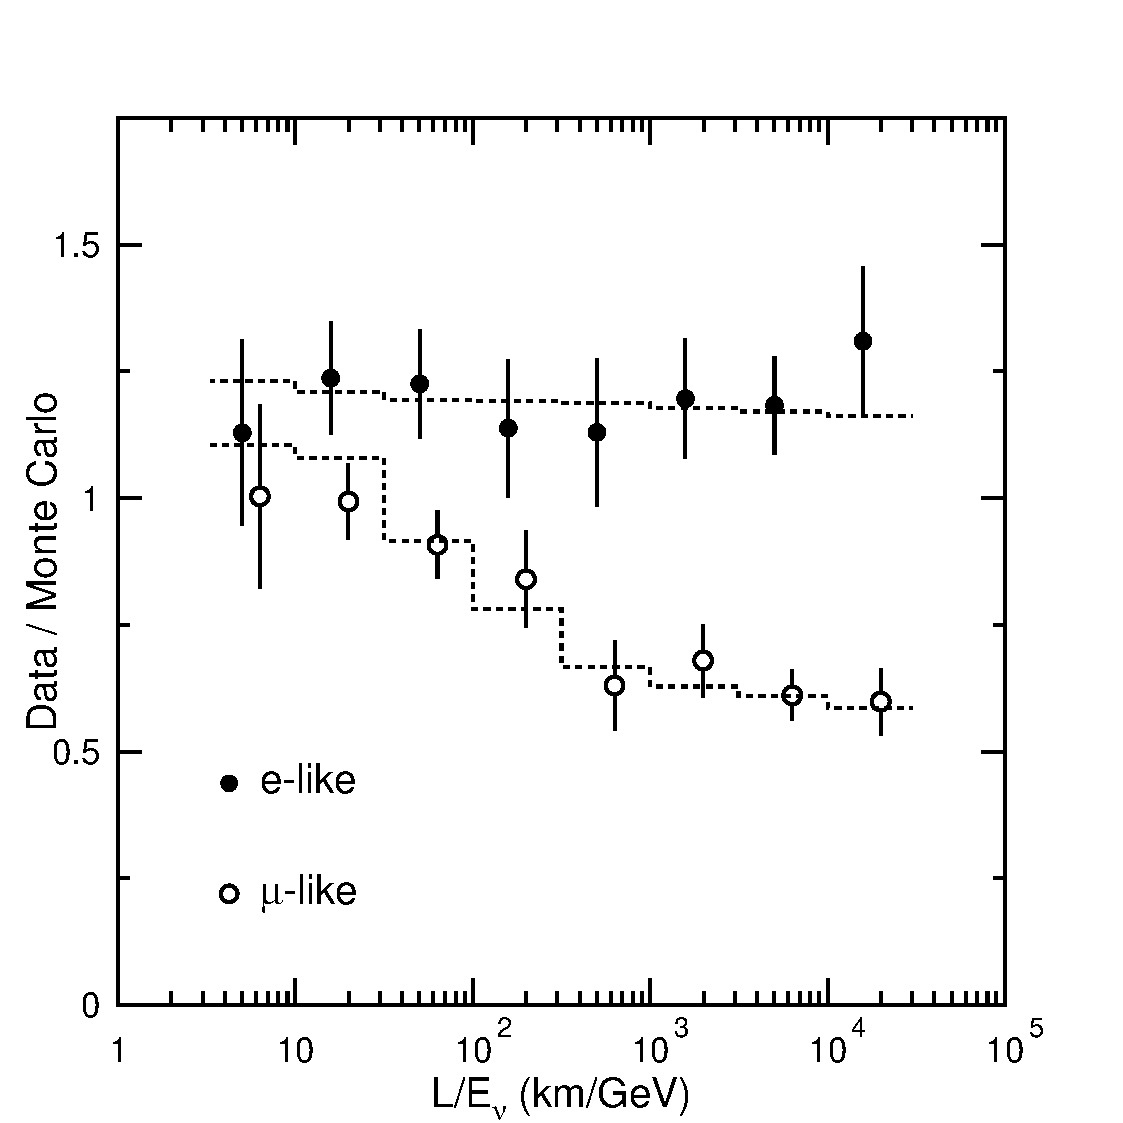
\includegraphics[width=0.7\linewidth]{images/super_k_emu_flux.pdf}
  \caption[Rapports des taux de neutrinos observé sur prédit en l'absence d'oscillation en fonction de $L/E_\nu$]{Rapports du taux de neutrinos observé sur le taux associé à la prédiction ne tenant pas compte du mécanisme d'oscillation: pour les candidats $\nu_e$ (points noirs) et $\nu_\mu$ (points blancs) en fonction de $L/E_\nu$. Les lignes en pointillés représentent les prédictions faisant intervenir l'oscillation $\nu_\mu \leftrightarrow \nu_\tau$ avec un angle de mélange à $\textrm{sin}^2(2\theta) = 1$. La décroissance du flux d'événements muoniques en $L/E_\nu$ a constitué une des premières preuves en faveur du mécanisme d'oscillations. (source : \cite{Fukuda:1998mi})}
  \label{fig:super_k_emu_flux.pdf}
\end{figure}

}

\bigbreak

Le rapport des flux $\phi(\nu_\mu + \overline{\nu}_\mu)/\phi(\nu_e + \overline{\nu}_e)$ était estimé à $\sim 2$ par des prédictions théoriques. L'avantage de cette observable est que l'incertitude sur la normalisation absolue du flux de neutrino qui est dominante devant toutes les autres, n'intervient pas ici. Ce rapport a été mesuré par Super-Kamiokande en observant l'état final de l'interaction par courants chargés des neutrinos sur des noyaux :

\begin{equation}
    \nu_l + N \rightarrow l + X,
\end{equation}

\bigbreak

\noindent
où $l$ est un lepton électronique ou muonique. L'identification du lepton a été établie en analysant la façon dont les photons sont dispersés autour de l'anneau Tcherenkov. Finalement, le rapport de flux qui a été mesuré ne s'élève qu'à environ 60\% de la prédiction \cite{Fukuda:1998mi}. De plus, l'information sur la direction de propagation du neutrino qui est fournie par la position de l'anneau a permis de trier les événements par distance de propagation. En effet, un neutrino créé dans l'atmosphère juste au-dessus du détecteur ne parcourt qu'une vingtaine de kilomètres, alors que s'il est émis depuis l'atmosphère de l'autre côté de la terre, il peut en parcourir jusqu'à 10000. Le mécanisme d'oscillation, qui est présenté dans la section suivante, fait intervenir le rapport distance de propagation sur énergie du neutrino : $L/E_\nu$. L'évolution du flux de neutrinos en $L/E_\nu$ (présenté sur la figure \ref{fig:super_k_emu_flux.pdf}) a fourni une première preuve en faveur du mécanisme d'oscillation.\\

La complétion du puzzle des oscillations de neutrinos est finalement venue de l'Observatoire de neutrinos de Sudbury au Canada, qui en 2002 a utilisé un détecteur Tcherenkov avec $\SI{1}{kt}$ d'eau lourde. Cette composition a offert la capacité d'observer des neutrinos via trois canaux :

\begin{itemize}[label=\textbullet]
    \item Par interaction d'un neutrino électronique sur un noyau de deutérium invoquant un courant chargé : $\nu_e + d \rightarrow p + p + e^-$, où l'énergie du neutrino est principalement emportée par l'électron ;
    \item Par diffusion inélastique d'un neutrino (avec n'importe quelle saveur active) sur un deutérium : $\nu_l + d \rightarrow \nu_x + p + n$, qui permet de normaliser le flux total de neutrino ;
    \item Et par diffusion élastique sur un électron, la réaction déjà utilisée par Super-Kamiokande.\\
\end{itemize}

%\bigbreak

La diffusion inélastique sur le deutérium présentait un défi expérimental majeur, car dans cette réaction seul le neutron est détectable, donc des exigences sévères sur la radiopureté de l'appareillage ont été requises. Puisque l'énergie seuil de cette réaction est à $\SI{2,2}{MeV}$, le flux de neutrinos issus du $^{8}B$ a pu être mesuré. Finalement, le flux obtenu par la diffusion inélastique s'est montré en accord avec la prédiction du SSM, prouvant que le nombre de neutrinos émis par le soleil est bien conservé \cite{Aharmim:2011vm}. Par ailleurs, le canal $\nu_e + d \rightarrow p + p + e^-$ a confirmé le déficit de flux de neutrino électroniques. SNO a donc été capable de démontrer le phénomène de conversion de saveur.\\

Ces deux expériences, Super-Kamiokande et SNO, auront été récompensées par la plus haute distinction en physique avec le prix Nobel de 2015 attribué à Takaaki Kajita et Arthur B. McDonald \og \textit{for the discovery of neutrino oscillations, which shows that neutrinos have mass} \fg{}. Néanmoins à l'époque où les résultats de SNO sont parus (2002), l'hypothèse des oscillations de saveur des neutrinos n'était pas la seule en mesure d'expliquer les effets observés. En réalité, les anomalies mesurées par SNO et Super-K. sont la conséquence de l'effet MSW traitant la conversion de saveur par des transitions adiabatiques des états de masse des neutrinos qui dépendent de la densité d'électron du milieu dans lequel ils se propagent (cf. figure \ref{fig:MSW_and_solar_neutrinos.png})\footnote{Alexei Yuryevich Smirnov ("S" de MSW) raconte dans \cite{Smirnov:2016xzf} qu'en 1986 à la conférence de Moriond, Albert Messiah l'aurait interpelé sur le fait d'avoir employé pendant sa présentation le terme d'\og oscillation \fg{} pour désigner l'effet MSW qui intervient dans la transformation des neutrinos solaires. Après que Smirnov lui ait répondu qu'il corrigerait cette terminologie, Messiah aurait commenté \og \textit{No way..., now this confusion will stay forever} \fg{}. Et en effet, la confusion s'est propagée jusque dans la désignation du prix Nobel! Cela montre à quel point il est délicat de changer la terminologie une fois que les idées ont été installées dans la culture.}. C'est l'expérience KamLAND, un détecteur doté de 1000 tonnes de liquide scintillateur placé sur l'ancien site de Kamiokande, qui va lever l'ambiguïté en mesurant l'oscillation des neutrinos générés par 55 réacteurs nucléaires à une distance moyenne de $\SI{150}{km}$ \cite{Gando:2013nba} : le motif d'oscillation est clairement visible sur la figure \ref{fig:KamLAND_spectrum.pdf}.\\

\afterpage{

\begin{figure}[h!]
\centering
\includegraphics[width=0.8\linewidth]{images/MSW_and_solar_neutrinos.png}
\caption[Anomalie de flux de neutrinos solaires en fonction de l'énergie]{Anomalie de flux de neutrinos solaires en fonction de l'énergie. Les points représentent les rapports de flux de neutrinos solaires mesurés sur la prédiction sans oscillation (les résultats de l'expérience italienne, Borexino, sont inclus). La bande grise représente la prédiction du flux prenant en compte le mécanisme d'oscillation et l'effet MSW. En dessous d'$\SI{1}{MeV}$ le déficit de flux est dominé par le mécanisme d'oscillation de saveur dans le vide, tandis que la chute du flux autour de $\SI{4}{MeV}$ est expliqué par la transition adiabatique des neutrinos qui se retrouvent tous sur l'état de masse $\nu_2$ en sortant du soleil. La probabilité d'être détecté sur terre est donc finalement donnée par la projection $|\left< \nu_e | \nu_2 \right>| = \textrm{sin}^2(2\theta_{12}) \simeq 30 \%$. (source : \cite{Franco:2013zwa})}
\label{fig:MSW_and_solar_neutrinos.png}
\end{figure}

\begin{figure}[h!]
\centering
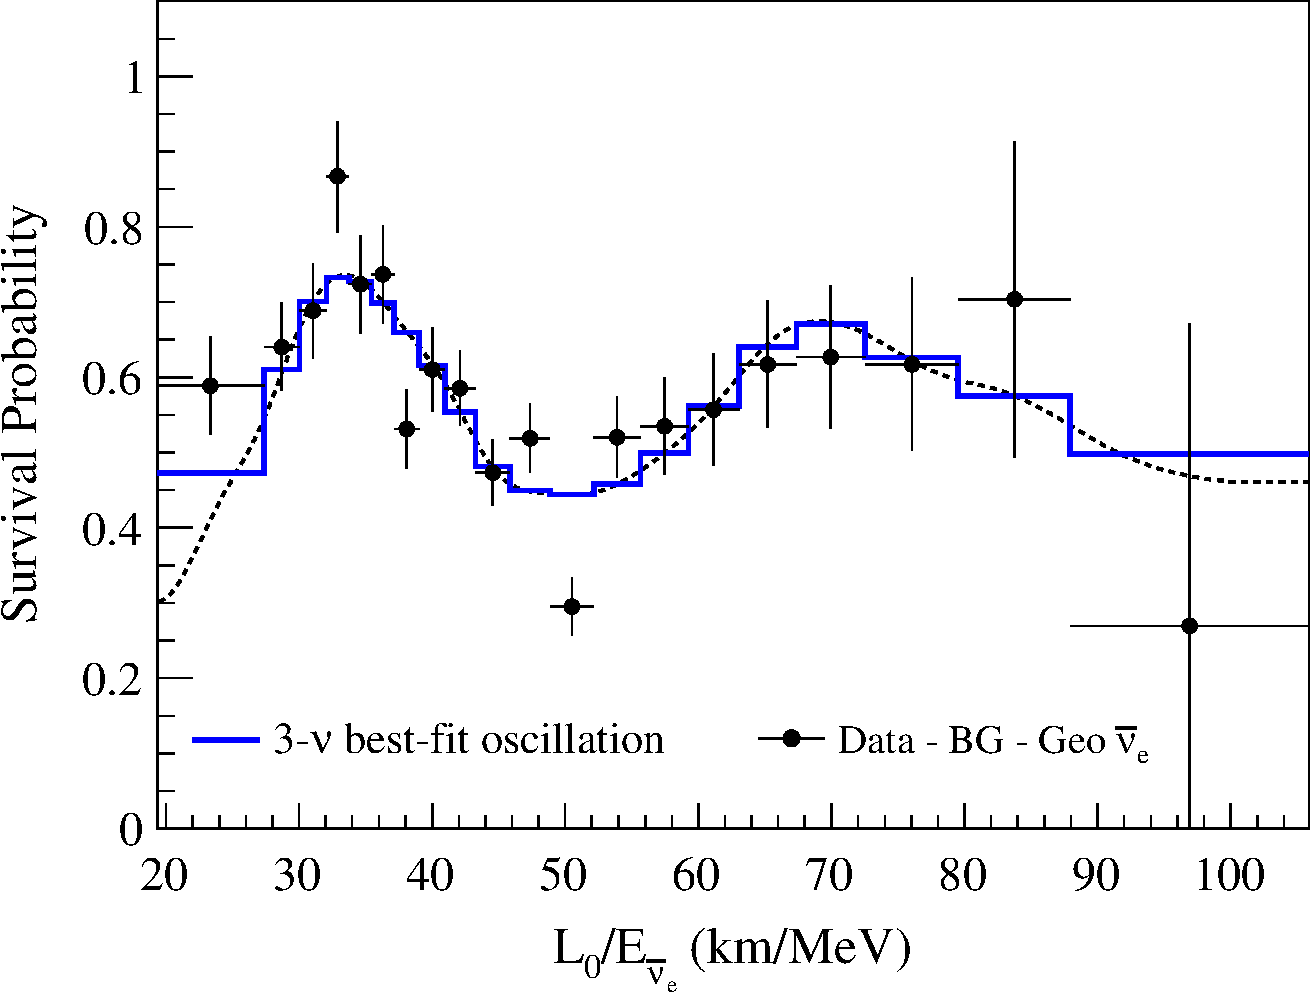
\includegraphics[width=0.8\linewidth]{images/KamLAND_spectrum.pdf}
\caption[Évolution du flux d'antineutrinos en fonction du rapport $L/E_\nu$ mesuré par KamLAND]{Évolution du flux d'antineutrinos en fonction du rapport $L/E_\nu$ mesuré par KamLAND. Les points noirs représentent le flux d'antineutrinos issus des 55 réacteurs situés à différentes distances du détecteur. La courbe pointillée et l'histogramme bleu représentent la prédiction ajustée avec les paramètres fournis par le mécanisme d'oscillation. (source : \cite{Gando:2013nba})}
\label{fig:KamLAND_spectrum.pdf}
\end{figure}

\clearpage

}

L'ensemble de ces résultats a finalement convaincu la communauté scientifique à adopter le modèle d'oscillation dans le vide ainsi que le mécanisme de transition des états de masse dans la matière. Cette approbation vient de pair avec le fait de considérer les neutrinos massifs, qui à l'origine n'avait pas été prévu dans le Modèle Standard. Puisque l'oscillation des neutrinos dans le vide constitue un point central de l'expérience \textsc{Stereo}, ce phénomène est brièvement introduit dans la section suivante.

\bigbreak

\subsection{Mélange des saveurs leptoniques}

% rise of the pmns paradigm

L'oscillation des neutrinos dans le vide est un phénomène de mécanique quantique qui se manifeste grâce à l'existence d'états propres de masse (ou de propagation) distincts des états propres d'interaction (ou de saveur). Ces deux bases sont reliées par une matrice de rotation nommée PMNS :

\begin{equation}
\left( \begin{matrix}
    \nu_e \\
    \nu_\mu \\
    \nu_\tau
\end{matrix} \right) = U_{PMNS} \left( \begin{matrix}
    \nu_1 \\
    \nu_2 \\
    \nu_3
\end{matrix} \right) = \left( \begin{matrix}
    U_{e1} & U_{e2} & U_{e3} \\
    U_{\mu 1} & U_{\mu 2} & U_{\mu 3} \\
    U_{\tau 1} & U_{\tau 2} & U_{\tau 3}
\end{matrix} \right) \left( \begin{matrix}
    \nu_1 \\
    \nu_2 \\
    \nu_3
\end{matrix} \right),
\end{equation}

\bigbreak

où les états propres d'interaction ($\nu_e$, $\nu_\mu$ et $\nu_\tau$) et les états propres de propagation ($\nu_1$, $\nu_2$ et $\nu_3$) sont reliés par la matrice unitaire $U_{PMNS}$. En théorie des champs, les états $\nu_e(x)$, $\nu_\mu(x)$ et $\nu_\tau(x)$ décrivent les neutrinos à hélicité gauche qui se couplent par interaction faible via les courants chargés aux électrons, aux muons et aux leptons tau respectivement; tandis que $\nu_1(x)$, $\nu_2(x)$ et $\nu_3(x)$ sont chacun associé à une masse $m_1$, $m_2$ et $m_3$. Une conséquence de ce mélange de saveurs est que les neutrinos qui se couplent à un lepton par courant faible chargé s'expriment comme une superposition cohérente d'états de masse :

\begin{equation}
    \mathcal{L}_{CC} = \frac{g}{\sqrt{2}} \sum_\mu W_\mu^- \sum_{\alpha = \{ e,\mu,\tau \}} \overline{l}_\alpha(x') \gamma^\mu \nu_\alpha(x) + \textrm{h.c.} =  \frac{g}{\sqrt{2}} \sum_\mu W_\mu^- \sum_{\alpha = \{ e,\mu,\tau \}} \overline{l}_\alpha(x') \gamma^\mu \sum_{i = \{ 1,2,3 \} } U_{\alpha i} \nu_i(x) + \textrm{h.c.},
\end{equation}

\bigbreak

où $\overline{l}_\alpha(x')$ sont les champs associés aux leptons chargés, $W^-_\mu$ représente le boson vecteur de l'interaction faible (courant chargé) et h.c. les termes hermitiens conjugués. À noter que seuls les leptons d'hélicité gauche interviennent dans ce Lagrangien. Le phénomène d'oscillation trouve son origine dans la présence de la matrice de passage $U_{\alpha i}$, car lorsque les neutrinos se propagent, ils sont projetés dans la base des états propres de masse, et quand vient le moment d'interagir avec un lepton $\alpha$, la probabilité est pondérée par le terme de matrice $U_{\alpha i}$ qui intervient dans le Lagrangien.\\

Puisque $U_{PMNS}$ est une matrice 3$\times$3 unitaire, il est possible de la paramétrer avec 3 angles de mélange et plusieurs phases complexes. Le nombre de phases dépend de la nature du neutrino : Dirac ou Majorana. Si les neutrinos sont des fermions de Dirac, alors il n'y a qu'une seule phase physique intervenant à propos de la violation de la symétrie CP. S'ils sont de Majorana cependant, deux phases supplémentaires doivent être ajoutées. La paramétrisation de la matrice PMNS peut s'écrire par le produit de trois matrices de rotation qui possèdent un \og angle de mélange \fg{} chacune ($\theta_{23}$, $\theta_{13}$ et $\theta_{12}$), où la deuxième fait intervenir la phase de violation CP $\delta_{CP}$:

\begin{equation}
    U_{PMNS} = \left( \begin{matrix}
        1 & 0 & 0\\
        0 & c_{23} & s_{23} \\
        0 & -s_{23} & c_{23}
    \end{matrix} \right) \left( \begin{matrix}
        c_{13} & 0 & s_{23}e^{-i\delta_{CP}}\\
        0 & 1 & 0 \\
        -s_{13}e^{i\delta_{CP}} & 0 & c_{23}
    \end{matrix} \right) \left( \begin{matrix}
        c_{12} & s_{12} & 0\\
        -s_{12} & c_{12} & 0 \\
        0 & 0 & 1
    \end{matrix} \right) P_\textrm{Majorana},
\end{equation}

\bigbreak

avec $c_{ij}$ et $s_{ij}$ qui signifient $\textrm{cos}(\theta_{ij})$ et $\textrm{sin}(\theta_{ij})$ respectivement. $P_\textrm{Majorana}$ est une matrice diagonale qui vaut l'identité si les neutrinos sont de Dirac, sinon elle fait intervenir deux phases supplémentaires. Les phases de Majorana sont cependant ignorées dans la discussion qui suit, car celles-ci n'interviennent pas dans les probabilités d'oscillation des neutrinos. La section suivante est consacrée à l'introduction de la probabilité d'oscillation.\\


%\bigbreak
%
%\begin{itemize}
%    \item formalisme mélange des saveurs (PMNS)
%    \item réécriture du lagrangien CC suivant les mass eigen states
%    \item symétries, invariances
%    \item paramétrisation (angle, delta m, phase CP, phases majorana)
%\end{itemize}


\bigbreak

\subsection{Oscillation des neutrinos dans le vide}

Dans le cadre d'un projet expérimental qui vise à mesurer les effets d'oscillation de neutrinos, la description des neutrinos peut être établie en trois étapes : création, propagation et détection. La première concerne la production de neutrinos suivant un état de saveur bien déterminé: $\alpha$. Dès lors que le neutrino se propage, il est projeté dans la base des états de masses. À l'instant de l'émission, $t = 0$, la conversion est déterminée par la matrice PMNS :

\begin{equation}
    \left|\nu(t = 0)\right> = \left|\nu_\alpha\right> = \sum_i U_{\alpha i}^* \left|\nu_i\right>.
\end{equation}

La seconde étape concerne l'évolution de l'état du neutrino lorsqu'il se propage. Chaque $\left|\nu_i\right>$ est un état propre du Hamiltonien (dans le vide) dont l'évolution est conduite par une phase $e^{iE_it}$, où $E_i = \sqrt{p^2 + m_i^2}$\footnote{on se place dans les unités de Planck pour simplifier les expressions : $c \doteq 1$, $\hbar \doteq 1$.} qui fait intervenir la masse du neutrino d'état propre $i$. Cette dernière modifie l'état de départ comme suit:

\begin{equation}
    \left|\nu(t)\right> = \sum_i U_{\alpha i}^* e^{iE_it} \left|\nu_i\right> = \sum_\beta \left|\nu_\beta\right> \sum_i U_{\beta i} U_{\alpha i}^* e^{iE_it},
\end{equation}

\bigbreak

où la somme sur $\beta$ permet de suivre la composition en termes d'états de saveur de $\left|\nu(t)\right>$. La détection de ce neutrino suivant une saveur spécifique est finalement déterminée par la projection $\left< \nu_\beta \right.\left|\nu(t)\right>$. L'amplitude de probabilité qu'un neutrino émis en $\alpha$ soit détecté en $\beta$ après un laps de temps $t$ s'écrit donc:

\begin{equation}
    P(\nu_\alpha \rightarrow \nu_\beta, t) = \left|\left< \nu_\beta \right.\left|\nu(t)\right>\right|^2 = \sum_i U_{\alpha i}^* U_{\beta i} \sum_j U_{\alpha j} U_{\beta j}^* \textrm{exp}\left(-(E_i - E_j)t\right).
\end{equation}

\bigbreak

En pratique les neutrinos sont ultra-relativistes ($p \gg m_i$ et $v \simeq c$), alors il est possible développer l'expression de l'énergie : $E_i = \sqrt{p^2 (1 + m_i^2/p^2)} \simeq p + m_i^2/(2E)$ en utilisant $E \simeq p$. L'argument de l'exponentielle peut être exprimé en fonction des différences de masses au carré $\Delta m_{ji}^2 \doteq m_j^2 - m_i^2$ :

\begin{equation}
    P(\nu_\alpha \rightarrow \nu_\beta, L) = \sum_i U_{\alpha i}^* U_{\beta i} \sum_j U_{\alpha j} U_{\beta j}^* \textrm{exp}\left(-\frac{\Delta m_{ji}^2}{2E} L\right),
\end{equation}

\begin{multline}
\label{eq:general_osc_prob}
    P(\nu_\alpha \rightarrow \nu_\beta, L) = \delta_{\alpha\beta} - 4 \sum_{i < j} \textrm{Re}\left[U_{\alpha i}U_{\beta i}^*U_{\alpha j}^*U_{\beta j} \right]\textrm{sin}^2\left(\frac{\Delta m^2_{ji} L}{4E} \right) \\
    + 2 \sum_{i < j} \textrm{Im}\left[U_{\alpha i}U_{\beta i}^*U_{\alpha j}^*U_{\beta j} \right]\textrm{sin}\left(\frac{\Delta m^2_{ji} L}{2E} \right),
\end{multline}

\bigbreak

où $L$ est la distance de propagation (égale à $t$ dans les unités naturelles). Il est important de noter que cette formulation a été obtenue avec plusieurs hypothèses simplificatrices. Par exemple, les états de masses qui se propagent ont été traités comme des ondes planes dont l'impulsion $p_i$ est parfaitement déterminée, et qui ont été définies comme égales entre elles. Si un développement plus rigoureux est nécessaire, celui-ci doit exploiter le formalisme de paquet d'ondes \cite{Smirnov:2016xzf}.\\

En vue obtenir la probabilité d'oscillation d'antineutrinos, il suffit de remplacer les éléments de matrice $U$ par $U^*$ et inversement. Pour pouvoir osciller, les états de masse des neutrinos doivent être non dégénérés ($\Delta m_{ji}^2 \neq 0$). La probabilité d'oscillation dépend finalement de cinq degrés de liberté : trois angles de mélanges $\theta_{12}$, $\theta_{23}$ et $\theta_{13}$, ainsi que deux différences de masses au carré (indépendantes). La phase de violation CP, qui traduit le fait que $P(\nu_\alpha \rightarrow \nu_\beta) \neq P(\overline{\nu}_\alpha \rightarrow \overline{\nu}_\beta)$, ne peut être sondée qu'en canal d'apparition (c'est-à-dire $\alpha \neq \beta$), car autrement \cite{Barger:1980jm} :

\begin{equation}
    P(\nu_\alpha \rightarrow \nu_\alpha) = 1 - 4 \sum_{i < j} \left| U_{\alpha i} U_{\alpha j}\right|^2 \textrm{sin}^2\left(\frac{\Delta m_{ji}^2 L}{4E} \right) = P(\overline{\nu}_\alpha \rightarrow \overline{\nu}_\alpha).
\end{equation}

\bigbreak

Cela s'explique par le fait que la transition $\nu_\alpha \rightarrow \nu_\alpha$ ne respecte pas seulement la symétrie CP, mais aussi CPT qui est régie par la relativité restreinte : donc pas de violation attendue. Afin d'étudier l'effet de la phase $\delta_{CP}$ sur l'oscillation des neutrinos, il faut introduire la quantité $\Delta P_{\alpha\beta} \doteq P(\nu_\alpha \rightarrow \nu_\beta ) - P(\overline{\nu}_\alpha \rightarrow \overline{\nu}_\beta )$ qui peut être obtenue d'après la partie imaginaire de l'Équation (\ref{eq:general_osc_prob}) \cite{Giganti:2017fhf} :

\begin{equation}
    \Delta P_{\alpha\beta} = \pm 16\ J\  \textrm{sin}\left(\frac{\Delta m_{21}^2 L}{4E} \right) \textrm{sin}\left(\frac{\Delta m_{31}^2 L}{4E} \right) \textrm{sin}\left(\frac{\Delta m_{32}^2 L}{4E} \right),
\end{equation}

\bigbreak

où le signe $\pm$ est déterminé par l'ordre des saveurs considérées : ($+$) si $\alpha, \beta, \gamma$ est une permutation paire de $e,\mu, \tau$, et ($-$) si c'est une permutation impaire. Le paramètre $J$ est défini comme étant l'invariant de \og \textit{Jarlskog} \fg{} dont l'expression est donnée par :

\begin{equation}
    J \doteq \textrm{Im}\left[U_{e1}U_{\mu 1}^* U_{e2}^* U_{\mu 2}\right] = \frac{1}{8}\ \textrm{cos}\theta_{13}\ \textrm{sin}(2\theta_{12})\ \textrm{sin}(2\theta_{13})\ \textrm{sin}(2\theta_{23})\ \textrm{sin}(\delta_{CP}).
\end{equation}

\bigbreak

Ainsi, pour parvenir à mesurer la phase de violation CP il faut que les trois angles de mélange soient non nuls et que les états de masse des neutrinos ne soient pas dégénérés. La mesure de $\delta_{CP}$ présente un intérêt particulier, car sa valeur permettrait d'apporter une réponse à la question : \textit{Pourquoi l'univers est-il essentiellement constitué de matière et non d'antimatière ?} Avant que des programmes expérimentaux ne se consacre à la question de $\delta_{CP}$, il a fallu attendre que l'ensemble des paramètres $\theta_{ij}$ et $\Delta m_{ij}^2$ aient été mesurés. C'est l'objet de la discussion dans la section suivante.

\bigbreak

\subsection{La physique expérimentale et les oscillations}

%

Chaque expérience qui vise à observer l'oscillation des neutrinos doit prendre en compte deux paramètres intervenant dans la probabilité $P(\nu_\alpha \rightarrow \nu_\beta )$ : la distance de propagation $L$ et l'énergie des neutrinos $E$. Afin de mesurer un motif d'oscillation, il y a principalement deux pratiques: soit l'expérience couvre plusieurs distances $L$ soit plusieurs énergies $E$. En effet, l'oscillation des neutrinos a un comportement sinusoïdal en $L/E$ dont la fréquence est dirigée par $\Delta m^2_{ij}$. Cependant, la résolution limitée en $E$ et en $L$ des instruments de mesure dégrade le signal après quelques périodes d'oscillation. En effet, lorsque $4E/L \gg \Delta m_{ij}^2$, l'argument du sinus carré est moyenné à cause des incertitudes :

\begin{equation}
    \textrm{sin}^2\left(\frac{\Delta m_{ij}^2 L}{4E} \right) \simeq \left< \textrm{sin}^2\left(x\right) \right> = \frac{1}{2}.
\end{equation}

\bigbreak

Il convient donc de se placer dans des conditions en $L$ et $E$ qui permettent d'être sensible aux premiers développements de l'oscillation. Puisque les paramètres $\Delta m_{21}^2$ et $\Delta m^2_{31}$ sont différents de deux ordres de grandeur, il est la plupart du temps possible de simplifier le mécanisme d'oscillation à deux saveurs :

\begin{equation}
\left( \begin{matrix}
    \nu_\alpha\\
    \nu_\beta
\end{matrix} \right) = \left( \begin{matrix}
    \textrm{cos} \theta & \textrm{sin}\theta \\
    - \textrm{sin} \theta & \textrm{cos}\theta
\end{matrix} \right) \left( \begin{matrix}
    \nu_1 \\
    \nu_2
\end{matrix} \right)
\end{equation}

\bigbreak

Les probabilités d'oscillation ont désormais des expressions ne faisant intervenir que  deux paramètres ($\theta$ et $\Delta m^2$) :

\begin{equation}
\label{eq:osc_two_flavors}
\begin{gathered}
    P(\nu_\alpha \rightarrow \nu_\beta ) = \textrm{sin}^2(2\theta)\textrm{sin}^2\left(\frac{\Delta m^2 L}{4E} \right) \textrm{ avec } \alpha \neq \beta ,\\
    P(\nu_\alpha \rightarrow \nu_\alpha ) = 1 - P(\nu_\alpha \rightarrow \nu_\beta ).
\end{gathered}
\end{equation}

\bigbreak

On remarque sur l'Équation (\ref{eq:osc_two_flavors}) que l'amplitude des oscillations est donnée par la valeur de $\theta$ tandis que $\Delta m^2$ donne la fréquence d'oscillation. À énergie fixée, le motif d'oscillation évolue avec la distance de propagation $L$ avec pour période $L_\textrm{osc} \doteq 4E/(\Delta m^2)$. En définitive, il est utile de travailler directement avec la probabilité d'oscillation suivante :

\begin{equation}
    P(\nu_\alpha \rightarrow \nu_\beta ) = \textrm{sin}^2(2\theta)\textrm{sin}^2\left(\frac{\pi L}{L_\textrm{osc}} \right) = \textrm{sin}^2(2\theta)\textrm{sin}^2\left(1,27 \frac{\Delta m^2(\SI{}{eV^2}) L(\SI{}{km})}{E (\SI{}{GeV})} \right)
\end{equation}

\bigbreak

Il est important de remarquer que cette expression n'est pas sensible au signe de $\Delta m^2$ (car $\textrm{sin}^2(x) = \textrm{sin}^2(-x)$) et que la valeur de l'angle $\theta$ ne peut être connue qu'à modulo $\pi/4$. Pour être sensible à ces grandeurs, il est nécessaire de considérer des effets du mécanisme d'oscillation avec trois saveurs. Cette formule à deux saveurs a été utilisée depuis des décennies, avant que les progrès instrumentaux n'atteignent un niveau de précision suffisant pour être sensible à des effets de second ordre. En particulier, le formalisme à deux saveurs s'est avéré suffisant pour décrire le résultat des expériences exploitant les neutrinos solaires ou atmosphériques. C'est d'ailleurs l'approche emprintée par \textsc{Stereo} pour mesurer l'oscillation vers un neutrino stérile (cf. section \ref{sec:sterile_exotic_solution}). Finalement, les paramètres mesurés avec les neutrinos solaires ($\Delta m^2_\textrm{sol} , \theta_\textrm{sol} $) correspondent aux états de masse 1 et 2, tandis que les neutrinos atmosphériques ($\Delta m^2_\textrm{atm} , \theta_\textrm{atm} $) sont identifiés avec les états 2 et 3:

\begin{equation}
    \Delta m^2_\textrm{sol} = \Delta m^2_{21} \ll \left| \Delta m_{32}^2 \right| = \Delta m^2_\textrm{atm}.
\end{equation}

\bigbreak

L'opérateur \og $\ll$ \fg{} provient du fait que la période d'oscillation $L_\textrm{osc}$ pour les neutrinos solaires ($\sim \SI{30}{km}$ à $E = \SI{1}{MeV}$) est plus grande que celle des neutrinos atmosphériques ($\sim \SI{1}{km}$ à $E = \SI{1}{MeV}$). La valeur absolue employée sur $\Delta m_{32}^2$ est là pour rappeler que la question de la hiérarchie de masse caractérisée par $m_1 > m_2 > m_3$ en hiérarchie \og normale \fg{} ($\Delta m_{32}^2 > 0$), contre $m_3 > m_1 > m_2$ en hiérarchie \og inversée \fg{} ($\Delta m_{32}^2 < 0$).\\

Les expériences qui exploitent les neutrinos atmosphériques sont caractérisées par des distances de propagation $L$ et des énergies $E$ telles que $\Delta m^2_\textrm{sol} L/E \ll 1$, permettant de négliger la contribution des neutrinos solaires. Il ne reste plus qu'une seule fréquence d'oscillation ($\Delta m^2_{32} \simeq \Delta m^2_{31}$) dont l'amplitude fait intervenir un angle effectif composé de $\theta_{23}$ et $\theta_{13}$:

\begin{equation}
\label{eq:general_atm_osc}
    P(\nu_\alpha \rightarrow \nu_\alpha ) = 1 - 4 \left|U_{\alpha 3}\right|^2 \left(1 - U_{\alpha 3}\right) \textrm{sin}^2\left(\frac{\Delta m^2_{32} L}{4E} \right) = 1 - \textrm{sin}^2\left(2 \theta_\textrm{eff} \right) \textrm{sin}^2\left(\frac{\Delta m^2_{32} L}{4E} \right)
\end{equation}

\bigbreak

Cette formule décrit bien le phénomène d'oscillations pour les neutrinos atmosphériques, mais aussi pour les expériences faisceau à longue distance ou encore les expériences auprès des réacteurs nucléaires. Puisque l'angle de mélange $\theta_{13}$ est faible devant $\theta_{23}$, il est possible de montrer que la probabilité de survie d'un neutrino muonique peut être approximée par :

\begin{equation}
    P(\nu_\mu \rightarrow \nu_\mu ) \simeq 1 - \textrm{sin}^2\left(2 \theta_{23} \right) \textrm{sin}^2\left(\frac{\Delta m^2_{32} L}{4E} \right)
\end{equation}

\bigbreak

C'est l'expression utilisée par les expériences exploitant les neutrinos atmosphériques pour la mesure de $\Delta m^2_{32}$ et $\theta_{23}$. Toujours à l'aide de la formule \ref{eq:general_atm_osc}, l'expression de la disparition des antineutrinos électroniques peut être dérivée:

\begin{equation}
    P(\overline{\nu}_e \rightarrow \overline{\nu}_e) = 1 - \textrm{sin}^2\left(2 \theta_{13} \right) \textrm{sin}^2\left(\frac{\Delta m^2_{32} L}{4E} \right)
\end{equation}

\bigbreak

Cette relation a été employée par les expériences exploitant des neutrinos produits par des réacteurs à courte distance (comme Double Chooz ou Daya Bay) pour mesurer l'angle de mélange le plus faible : $\theta_{13}$. Par ailleurs, si on considère que les valeurs typiques de $L$ et $E$ sont telles que $\Delta m^2_\textrm{atm} L/E \gg 1$, mais qu'en revanche $\Delta m^2_\textrm{sol} L/E \gtrsim 1 $, l'oscillation est conduite cette fois par $\Delta m^2_\textrm{sol} = \Delta m^2_{21}$. Avec l'approximation à deux saveurs, la probabilité de survie des neutrinos électronique est :

\begin{equation}
\label{eq:two_flavor_solar}
    P(\nu_e \rightarrow \nu_e) = P(\overline{\nu}_e \rightarrow \overline{\nu}_e) \simeq 1 - \textrm{sin}^2\left(2 \theta_{12} \right) \textrm{sin}^2\left(\frac{\Delta m^2_{21} L}{4E} \right)
\end{equation}

\bigbreak

Cette formule s'applique aux mesures obtenues par les expériences des neutrinos solaires à base énergie ($E < \SI{1}{MeV}$ sinon la disparition est due à l'effet MSW) bien que le mélange soit moyenné, car $\Delta m^2_\textrm{sol} L/E \gg 1 $, et par l'expérience KamLAND qui exploite les neutrinos de réacteur à grandes distances de propagation. Il est important de garder à l'esprit que ces expressions négligent les effets à 3 saveurs, qui doivent être prises en compte pour répondre aux exigences de précision des expériences contemporaines. Par exemple dans (\ref{eq:two_flavor_solar}), la réinsertion de $\theta_{13}$ permet d'avoir une expression plus précise :

\begin{equation}
    P(\nu_e \rightarrow \nu_e) = P(\overline{\nu}_e \rightarrow \overline{\nu}_e) = \left(1 - \textrm{sin}^2\left(2 \theta_{12} \right) \textrm{sin}^2\left(\frac{\Delta m^2_{21} L}{4E} \right)\right) \times \textrm{cos}^4\left(\theta_{13}\right) + \textrm{sin}^4\left(\theta_{13}\right).
\end{equation}

%Avec le recul, les expériences précurseurs qui ont mesurés des neutrinos provenant du soleil ont en fait mesuré l'oscillation moyennée :
%
%\begin{equation}
%    P(\nu_\alpha \rightarrow \nu_\alpha ) = 1 - \left\{ \textrm{sin}^2\left(2 \theta_{23} \right) + \textrm{sin}^2\left(2 \theta_{12} \right) \right\} \times \frac{1}{2} .
%\end{equation}

\subsection{État de l'art du modèle d'oscillations à 3 saveurs}

La mesure des cinq paramètres de la matrice PMNS ($\theta_{12}, \theta_{23}, \theta_{13}, \Delta m_{21}^2, \Delta m_{31}^2$) a été le fruit de développements expérimentaux qui se sont déroulés dans les deux dernières décennies. Une très large part des résultats, à l'exception de quelques anomalies qui sont décrites dans la section suivante, sont en faveur du modèle à trois neutrinos actifs qui se mélangent par le mécanisme d'oscillation paramétrisé par la matrice PMNS.\\

L'ajustement global de la matrice PMNS sur l'ensemble des données acquises a été effectué par plusieurs analyses depuis 2014. Les résultats issus de la dernière en date \cite{Esteban2017} sont présentés dans le Tableau \ref{tab:global_fit_PMNS}. Puisqu'à l'heure actuelle la question de la hiérarchie de masse n'a pas encore été tranchée, les résultats sont présentés dans les deux cas de figure. De plus, chaque incertitude est séparée en partie positive et négative, car les contraintes de l'ajustement ne sont pas symétriques. Chaque valeur représente l'écart type à $1\sigma$, mais il faut garder à l'esprit que l'erreur à $2\sigma$ ne peut être directement obtenue en échelonnant l'erreur à $1\sigma$ avec un facteur 2: il est nécessaire de faire intervenir les véritables distributions de probabilité.

\begin{table}[h!]
\begin{center}
\begin{tabular}{|c|c|c|}
\hline
Paramètre & Hiérarchie Normale & Hiérarchie Inversée \\
\hline
$\theta_{12} (^\circ)$ & $33.56^{+0.77}_{-0.75}$ & $33.56^{+0.77}_{-0.75}$\\
\hline
$\theta_{23} (^\circ)$ & $41.46^{+1.5}_{-1.2}$ & $50.0^{+1.1}_{-1.4}$\\
\hline
$\theta_{13} (^\circ)$ & $8.46^{+0.15}_{-0.15}$ & $8.49^{+0.15}_{-0.15}$\\
\hline
$\Delta m^2_{21} (\SI{}{eV^2})$ & $7.50^{+0.19}_{-0.17} \times 10^{-5}$ & $7.50^{+0.19}_{-0.17} \times 10^{-5}$\\
\hline
$\Delta m^2_{31} (\SI{}{eV^2})$ & $2.524^{+0.039}_{-0.040} \times 10^{-3}$ & \\
\hline
$\Delta m^2_{32} (\SI{}{eV^2})$ & & $-2.514^{+0.038}_{-0.041} \times 10^{-3}$\\
\hline
\end{tabular}
\caption[Paramètres de la matrice PMNS déterminés par l'analyse globale des résultats des expériences neutrinos]{Paramètres de la matrice PMNS déterminés par l'analyse globale des résultats des expériences neutrinos \cite{Esteban2017}. Les valeurs sont présentées pour les deux cas de hiérarchie de masse.}
\label{tab:global_fit_PMNS}
\end{center}
\end{table}

%\subsubsection*{L'analyse globale PMNS}
%
%\begin{itemize}
%    \item Tableau des résultats
%    \item Global fit ?
%    \item Next step ? T2K Nova Dune ?
%\end{itemize}

\bigbreak

\section{Anomalies expérimentales}

\subsection{Anomalie auprès des réacteurs}
\label{sec:anomaly_reacteur}

\subsubsection*{Processus de production des antineutrinos}

Les réacteurs nucléaires constituent une des sources d'antineutrinos les plus intenses maîtrisées par l'Homme. En effet, le processus de fission démarre d'un combustible enrichi en uranium 235 ($\ce{^{235}U}$), qui génère des noyaux instables et très riches en neutrons subissant des désintégrations $\beta^-$. La fission d'un noyau d'$\ce{^{235}U}$ peut aboutir sur de multiples paires de noyaux plus légers comme le montre les distributions sur la figure \ref{fig:nuclear_out_fission.png}. Pour illustrer la production d'antineutrinos électroniques, un exemple typique est la réaction :

\afterpage{

\begin{figure}[h!]
  \centering
  \includegraphics[width=0.7\linewidth]{images/nuclear_out_fission.png}
  \caption[Répartition en masse des produits de fission des isotopes fissibles présents dans un réacteur nucléaire]{Répartition en masse des produits de fission des isotopes fissibles présents dans un réacteur nucléaire : $\ce{^{235}U}$, $\ce{^{239}Pu}$, $\ce{^{238}U}$ et $\ce{^{241}Pu}$. La fission de ces noyaux génère la production d'un couple de deux noyaux plus légers. Les effets de structure nucléaire impliquent une fission asymétrique avec une distribution de masse du produit de fission le plus lourd essentiellement indépendante de l'isotope de départ. La sensibilité à cet isotope se retrouve alors dans la distribution de masse du noyau le plus léger. (source : \cite{PhysRevC.88.014605})}
  \label{fig:nuclear_out_fission.png}
\end{figure}

\begin{figure}[h!]
  \centering
  \includegraphics[width=0.7\linewidth]{images/exemple_fission_process.png}
  \caption[Exemple de fission d'un noyau d'$\ce{^{235}U}$]{Exemple de fission d'un noyau d'$\ce{^{235}U}$ en $\ce{^{140}Ba}$ et $\ce{^{94}Kr}$. Les désintégrations $\beta^-$ successives de ces deux derniers isotopes sont responsables de l'émission d'antineutrinos électroniques. Par ailleurs, les neutrons produits par la fission de l'$\ce{^{235}U}$ induisent de nouvelles fissions sur d'autres isotopes lourds : la réaction en chaine est amorcée.}
  \label{fig:exemple_fission_process.png}
\end{figure}

\clearpage

}

\begin{equation}
    \ce{^{235}U} + n \rightarrow \ce{^{140}Ba} + \ce{^{94}Kr} + 2n,
\end{equation}

\bigbreak

qui libère environ $\SI{200}{MeV}$. Les noyaux de $\ce{^{140}Ba}$ et de $\ce{^{94}Kr}$ sont riches en neutron et décroissent rapidement par $\beta^-$. La chaine de décroissance est représentée sur la figure \ref{fig:exemple_fission_process.png} et montre que les désintégrations beta successives donnent naissance à sept antineutrinos. Les neutrinos peuvent aussi provenir de la fission de $\ce{^{239}Pu}$, mais cet isotope n'est pas présent à l'origine dans le combustible. Il est créé à mesure que le combustible se consumme (\og \textit{Burn up} \fg{}), par une transition provoquée à l'origine par la capture d'un neutron rapide sur l'$\ce{^{238}U}$ :

\begin{equation}
    \ce{^{238}U} + n \rightarrow \ce{^{239}U} \rightarrow \ce{^{239}Np} + e^- + \overline{\nu}_e \rightarrow \ce{^{239}Pu} + e^- + \overline{\nu}_e.
\end{equation}

\bigbreak

Le $\ce{^{239}Pu}$ qui s'accumule est lui aussi affecté par l'environnement chargé en neutrons, et se transforme par captures successives en $\ce{^{241}Pu}$. Les deux isotopes $\ce{^{239}Pu}$ et $\ce{^{241}Pu}$ sont fissibles, donc leur contribution relative au flux d'antineutrinos augmente avec le temps. De plus, les neutrinos peuvent être générés par la fission d'$\ce{^{238}U}$ induite par des neutrons rapides. L'évolution de la fraction d'isotopes fissibles ($\ce{^{235}U}$, $\ce{^{238}U}$, $\ce{^{239}Pu}$ et $\ce{^{241}Pu}$) dans un c\oe ur de réacteur est présentée sur la figure \ref{fig:nu_flux_burnup.png}. Les neutrinos issus de l'$\ce{^{235}U}$ sont largement majoritaires, mais à mesure que le combustible se consume, la contribution du $\ce{^{239}Pu}$ devient non négligeable.\\

Pour résumer, les réacteurs nucléaires sont des sources pures d'antineutrinos électroniques avec des énergies de quelques MeVs, dont le flux total est d'environ $10^{20} \SI{}{\nu/s/GW_{th}}$. La prédiction des spectres antineutrinos est donc la résultante de milliers de branches de désintégrations $\beta^-$ déterminées par les produits de fission. Les défis majeurs de cette tâche résident dans le traitement d'ingrédients de physique nucléaire complexes comme la forme spectrale de chaque transition $\beta^-$, le suivi en temps de la composition du c\oe ur du réacteur, ou encore l'incomplétude des bases de données nucléaires pour le noyaux les plus instables.\\

La contribution des quatre principaux isotopes au flux d'antineutrinos évolue avec le temps. Le flux total d'antineutrinos émis est obtenu grâce à la relation suivante :

\begin{equation}
    \phi_\nu^\textrm{em}(E,t) = \frac{P_{th}(t)}{\sum_k \alpha_k (t) E_k} \sum_k \alpha_k (t) S_k(E),
\end{equation}

\bigbreak

avec $P_{th}$ la puissante thermique dégagée par le c\oe ur, $E_k$ l'énergie libérée par la fission de l'isotope $k$, $\alpha_k$ la fraction du nombre de fissions portée par l'isotope $k$ et $S_k$ le spectre en énergie des antineutrinos issus de la fission de l'isotope $k$. La puissance thermique est mesurée en continu, tandis que $E_k$ est fournie par les bases de données nucléaires. L'évolution de la fraction isotopique $\alpha_k$ est estimée par des simulations qui modélisent la transmutation des matériaux dans les c\oe urs des réacteurs. Enfin, les spectres antineutrino $S_k(E)$ sont déterminés par calcul, et constituent les sources dominantes d'incertitudes sur  $\phi_\nu^\textrm{em}$.\\

La réaction la plus utilisée pour détecter les neutrinos de réacteurs est la décroissance beta inverse, qui a déjà été mentionnée dans la partie historique. Celle-ci possède un seuil en énergie neutrino à $E_{IBD} \simeq \SI{1.8}{MeV}$ qui doit être pris en compte pour discuter la contribution de chaque isotope au flux d'antineutrinos détectables. Désormais, lorsqu'il est question du flux d'antineutrinos provenant d'un réacteur nucléaire, la quantité en jeu est :

\afterpage{

\begin{figure}[h!]
  \centering
  \includegraphics[width=0.7\linewidth]{images/nu_flux_burnup.png}
  \caption[Évolution de la contribution relative au nombre total de fissions en fonction du \textit{burn up}]{Évolution de la contribution relative au nombre total de fissions en fonction du \textit{burn up}. Les conditions initiales du combustible sont celles d'un réacteur commercial en début de cycle, après rechargement d'1/3 de son combustible (enrichi à 3,5\% en $\ce{^{235}U}$). (source : \cite{An:2016srz})}
  \label{fig:nu_flux_burnup.png}
\end{figure}

\begin{table}[h!]
  \begin{center}
    \begin{tabular}{|c|c|c|}
    \hline
      Isotope fissible & $\ce{^{235}U}$  & $\ce{^{239}Pu}$\\
      \hline
      \hline
      $E_k$ & $\SI{202}{MeV}$ & $\SI{211}{MeV}$\\
      \hline
      $\left< E_\nu \right>$ ($E_\nu > \SI{1.8}{MeV}$) & $\SI{2.94}{MeV}$ & $\SI{2.84}{MeV}$\\
      \hline
      $N_{\nu/\textrm{fission}}$ ($E_\nu > \SI{1.8}{MeV}$) & 1,92 & 1,45\\
      \hline
      $\left<\sigma_\nu^\textrm{int}\right>$ & $\simeq 3,20 \times 10^{-43} \SI{}{cm^2}$ & $\simeq 2,76 \times 10^{-43} \SI{}{cm^2}$ \\
      \hline
    \end{tabular}
  \end{center}
  \caption[Propriétés des principaux isotopes fissibles contribuant au flux d'antineutrinos détectables]{Propriétés des principaux isotopes fissibles contribuant au flux d'antineutrinos détectables. $\sigma_\nu^\textrm{int}$ représente la section efficace d'interaction par IBD des neutrinos moyennée sur l'ensemble du spectre à l'émission $S_k(E)$ depuis le seuil en énergie de l'IBD.}
    \label{tab:iso_properties}
\end{table}

}

\begin{equation}
\begin{gathered}
    \phi^\textrm{em}_\nu(t) = \int_{E_{IBD}}^{+\infty} \phi^\textrm{em}_\nu(E, t) dE = \frac{P_{th}(t)}{\sum_k \alpha_k (t) E_k} \sum_k \alpha_k (t) \int_{E_{IBD}}^{+\infty} S_k(E) dE,\\
    \phi^\textrm{em}_\nu(t) = \frac{P_{th}(t)}{\sum_k \alpha_k (t) E_k} \sum_k \alpha_k (t) N_k^{\nu/\textrm{fission}},
\end{gathered}
\end{equation}

\bigbreak

où $N_k^{\nu/\textrm{fission}}$ est le nombre d'antineutrinos détectables générés par fission de l'isotope $k$. Les paramètres des deux principaux isotopes sont rassemblés dans le Tableau \ref{tab:iso_properties}. Pour une même puissance thermique libérée, le rapport du nombre de neutrinos détectés issus de l'$\ce{^{235}U}$ contre le $\ce{^{239}Pu}$ peut s'exprimer ainsi :

\begin{equation}
    \frac{N_\nu^\textrm{det} (\ce{^{235}U})}{N_\nu^\textrm{det} (\ce{^{239}Pu})} = \frac{N_{\nu/\textrm{fission}} \left<\sigma_\nu^\textrm{int}\right>}{E_k} (\ce{^{235}U}) \times \frac{E_k}{N_{\nu/\textrm{fission}} \left<\sigma_\nu^\textrm{int}\right>} (\ce{^{239}Pu}) = \frac{211}{202} \times \frac{1,92}{1,45} \times \frac{3,20}{2,76} = 1,60.
\end{equation}

\bigbreak

Le nombre de neutrinos détectés issus de la fission d'$\ce{^{235}U}$ est 60 \% plus important que pour le $\ce{^{239}Pu}$. Cela signifie qu'au cours d'un cycle de fonctionnement (période pendant laquelle le réacteur fonctionne en continu avec un combustible), le nombre total d'antineutrinos détectés diminue ainsi que leur énergie moyenne. Cet effet a été observé pour la première fois au début des années 90 sur le réacteur de puissance Rovno en Russie \cite{Kuvshinnikov:1990ry}, et constitue aujourd'hui un pan de la physique appliquée des neutrinos sur la non-prolifération des armes atomiques.\\

\subsubsection*{Prédiction des spectres antineutrinos}

\afterpage{

%spectrum_component_U5.png
\begin{figure}[h!]
  \centering
  \includegraphics[width=0.7\linewidth]{images/spectrum_component_U5.png}
  \caption[Exemple de construction \textit{ab initio} du spectre antineutrino issu de la fission d'$\ce{^{235}U}$]{Exemple de construction \textit{ab initio} du spectre antineutrino issu de la fission d'$\ce{^{235}U}$. Chaque ligne symbolise une composante du spectre total (ligne bleue foncée). Les points représentent les spectres électron mesurés à l'ILL dans les années 80 \cite{Schreckenbach:1981wlm}. (source : \cite{Sonzogni:2015aoa})}
  \label{fig:spectrum_component_U5.png}
\end{figure}


}

%La physique fondamentale se consacre cependant à l'étude en absolu des flux d'antineutrinos issus des réacteurs nucléaires. 

L'anomalie trouve son origine dans les entrailles de $S_k(E)$. La détermination de cette quantité peut être établie par deux méthodes :

\begin{itemize}[label=\textbullet]
    \item $S_k(E)$ peut être construit en ajoutant la contribution de toutes les branches de décroissance beta de tous les fragments de fission. Cette technique requiert évidemment de connaître tous les rendements de produits de fission (quelle est la fréquence de production d'un isotope donné par fission ?), les temps de vie de ces derniers, les rapports d'embranchements des canaux de désintégration $\beta^-$, les extrémités (\og \textit{endpoints} \fg{}) des spectres $\beta^-$, et encore les formes des spectres antineutrino de chacun d'eux.
    \item Sinon les $S_k(E)$ sont accessibles en mesurant directement le spectre électron associé à l'isotope fissible $k$, puis en le convertissant en spectre antineutrino ($S_k(E)$). La correspondance directe $E_\nu = E_\textrm{endpoint} - E_e$, vérifiée au niveau de chaque branche bêta, est cependant perdue au niveau du spectre électron total mesuré. La procédure de conversion en neutrino devra donc faire appel à des approximations.
\end{itemize}

\bigbreak

Dans les deux cas, l'estimation des erreurs systématiques est cruciale pour établir une inférence avec les mesures directes des spectres antineutrino.\\

La méthode \textit{ab initio} décompose $S_k(E)$ de la façon suivante :

\begin{equation}
    S_k(E) = \sum_{f} A_{f}\times S_{f}(E) = \sum_{f} A_{f} \sum_{b} BR^b_{f} \times S^b_{f}(Z_{f}, A_{f}, E^b_{0, f}, E),
\end{equation}

\bigbreak

avec la somme sur $f$ qui représente chaque produit de fission avec l'activité prédite $A_{f}$, et la somme sur $b$ pour chaque rapport d'embranchement $BR^b_{f}$. Pour exemple, la décroissance de l'$\ce{^{235}U}$ fait intervenir $\sim 6000$ spectres $S^b_{f}$ : une représentation de ces composantes est dessinée sur la figure \ref{fig:spectrum_component_U5.png}. La forme de chaque branche $S^b_{f}$ est obtenue par des calculs théoriques qui font intervenir des facteurs de forme, ainsi que des facteurs de correction. Si ces quantités sont bien contrôlées pour les transitions autorisées (moment angulaire du système électron + neutrino : $L = 0$), elles présentent des dépendances complexes avec la structure du noyau pour les transitions interdites ($L \geq 1$).\\

\afterpage{

% ILL_beta_spectra.png

\begin{figure}[h!]
  \centering
  \includegraphics[width=0.7\linewidth]{images/ILL_beta_spectra.png}
  \caption[Spectres électrons associés à la fission de l'$\ce{^{235}U}$, du $\ce{^{239}Pu}$ et du $\ce{^{241}Pu}$ mesurés]{Spectres électrons associés à la fission de l'$\ce{^{235}U}$ (vert), du $\ce{^{239}Pu}$ (rouge) et du $\ce{^{241}Pu}$ (bleu), mesurés à l'ILL. (source : \cite{Lhuillier:2013qza})}
  \label{fig:ILL_beta_spectra.png}
\end{figure}


}

Les mesures des spectres électrons associés à la fission de l'$\ce{^{235}U}$, du $\ce{^{239}Pu}$ et du $\ce{^{241}Pu}$ ont été menées dans les années 1980 à l'ILL avec le spectromètre magnétique à haute résolution BILL \cite{Schreckenbach:WorkshoponBeyondThreeFamilyNeutrinoOscillations}. C'est cette approche qui fut la clé pour fournir des prédictions suffisamment précises (mieux que 10\%), pour être exploitables par les neutrinistes. Des échantillons sous forme de feuilles étaient irradiés près du c\oe ur du réacteur par le flux de neutrons thermiques environnant pendant des durées allant de $\sim 12\SI{}{h}$ à presque 2 jours. Les spectres électrons associés à l'$\ce{^{235}U}$ ont été mesurés à deux reprises en 1981 puis en 1985 (\cite{Schreckenbach:1981wlm} et \cite{Schreckenbach:1985ep}), tandis que ceux du $\ce{^{239}Pu}$ et du $\ce{^{241}Pu}$ en 1982 et 1989 respectivement (\cite{VonFeilitzsch:1982jw} et \cite{Hahn:1989zr}). La normalisation des spectres a été réalisée à l'aide de réactions de calibration $(n,\gamma)$ dont les sections efficaces sont bien connues. Les trois spectres exprimés en coups par fissions sont présentés sur la figure \ref{fig:ILL_beta_spectra.png}.\\

La conversion d'un spectre de décroissance beta vers spectre antineutrino peut être effectuée à partir de la relation $S_\nu(E) = S_e(E_0 - E)$ où $E_0$ est le \textit{end-point} du spectre Beta. Pour appliquer cette transformation sur les spectres mesurés à l'ILL, il est nécessaire de les décomposer en une superposition de spectres Beta. Les données mesurées à l'ILL ont donc été ajustées par une trentaine de spectres beta aussi appelés \og branches virtuelles \fg{} \cite{Vogel:2007du}. Les mesures directes des spectres antineutrino par les expériences Bugey 3 \cite{Achkar:1996rd} et Goesgen \cite{Zacek:1986cu} sont venues confirmer les prédictions des spectres et infirmer les hypothèses d'oscillation à courtes distances. Ces deux expériences ont marqué la fin de l'ère d'exploration des oscillations de neutrino essentiellement en aveugle. En effet à la fin des années 1990, le cadre des oscillations de neutrino avait été établi, du moins sommairement. L'étude des neutrinos atmosphériques avait conduit à l'attribution de  $\Delta m^2_\textrm{atm} \simeq 2-4 \times 10^{-3} \SI{}{eV^2}$, et la physique des neutrinos solaires pointait du doigt la zone $\Delta m^2_\textrm{sol} \sim 10^{-4} \SI{}{eV^2}$. Les expériences exploitant les antineutrinos de réacteurs se sont par conséquent tourné vers des configurations à $\sim \SI{1}{km}$ de la source, imposé par $\Delta m^2_\textrm{atm}$, pour la mesure de $\theta_{13}$ (avec les expériences Chooz ou Palo Verde par exemple), et des configurations sur des distances de $\sim \SI{100}{km}$, correspondant à $m^2_\textrm{sol}$, pour démontrer la validité de l'interprétation des observations des neutrinos solaires avec PMNS. Ce programme expérimental a été réalisé par KamLAND.\\

\bigbreak

\subsubsection*{Réévaluation des spectres antineutrino}

Au début des années 2010, la précision requise pour la mesure de $\theta_{13}$ a mené la communauté à s'intéresser de nouveau à la question des prédictions des spectres réacteur. Les travaux de Muller \textit{et al.} \cite{Mueller:2011nm} ont proposé une nouvelle estimation des spectres antineutrino qui repart de l'approche \textit{ab initio}. Les améliorations des bases de données nucléaires ont permis de reconstruire $\sim 90\%$ du spectre électron total à partir des seules transitions considérées comme  \og bien connues \fg{} (end-point, spin et parité bien mesurés, effet pandemonium\footnote{L'effet pandemonium est un 	biais sur les mesures des rapports d'embranchement d'une désintégration beta.} corrigé). Ces transitions permettent de rapprocher au mieux les distributions physiques de transitions bêta sous-jacentes du spectre total électron mesuré. Lorsque la transition est permise la conversion en neutrino est même exacte. La contribution manquante qui provient de noyaux inconnus et des incertitudes systématiques des bases de données nucléaires est ajustée à l'aide d'un ensemble de cinq branches effectives beta virtuelles. Les spectres antineutrino qui résultent de cette étude se sont retrouvés amplifiés d'un facteur de normalisation de $\sim +3,0 \%$. \\

%Cet excès trouve son origine dans deux effets indépendants dont l'un affecte la partie basse énergie du spectre et l'autre la haute énergie. À basse énergie, les corrections à la théorie de Fermi (qui interviennent dans $S_{f}^b$) sont linéaires branche par branche, mais pas sur la résultante du spectre total. L'application de ces corrections nécessitait l'emploi d'autres termes qui n'avaient pas été considérés à l'époque. Sinon, la partie haute énergie était affectée par une mauvaise distribution en charge des branches Beta fournies par les bases de données nucléaires de l'époque.\\

Par la suite, les études réalisées par Huber \cite{Huber:2011wv} ont confirmé la nécessité de corriger ce biais dans la procédure de conversion des spectres électron. De plus, bénéficiant des spectres électrons mesurés à l'ILL avec un binning plus fin et affichant une meilleure stabilité de la procédure de conversion, ces résultats sont devenus les prédictions des références connues sous le nom de \og spectres d'Huber \fg{}. Cependant, la prédiction associée aux neutrinos issus de l'$\ce{^{238}U}$ dont la fission est induite par des neutrons rapides, avaient été traitées dans la papier original de Mueller \textit{et al.} et se sont finalement retrouvées estampillées : prédictions de Mueller. Ainsi, lorsqu'il est question des prédictions des antineutrinos de réacteur issus de l'$\ce{^{235}U}$, l'$\ce{^{238}U}$, du $\ce{^{239}Pu}$ et du $\ce{^{241}Pu}$, la littérature fait référence à ces deux auteurs : spectres d'Huber-Mueller.\\

Par dessus ces biais sont ajoutés des termes correctifs tenant compte de la durée limitée de l'irradiation des échantillons lors des mesures à l'ILL dans les années 1980. Les échantillons soumis au flux de neutrons thermiques étaient irradiés sur une durée allant de 12 h à environ 2 jours, or les combustibles des réacteurs sont habituellement exposés pendant plusieurs dizaines de jours dans le cas des réacteurs de recherche, et plus d'un an dans le cas des réacteurs commerciaux. Les neutrinos détectés sont donc également issus de produits de fission dont la durée de vie dépasse la journée. Des facteurs dits \og hors équilibre \fg{} pour corriger cet effet n'avaient pas été considérés jusqu'alors. Ces derniers affectent la prédiction originale à hauteur de +1\%.\\

\afterpage{

% Gariazzo:2017fdh
% RAA_2017.png

\begin{figure}[h!]
  \centering
  \includegraphics[width=0.95\linewidth]{images/RAA_2017.png}
  \caption[Illustration de l'anomalie des antineutrinos de réacteur]{Illustration de l'anomalie des antineutrinos de réacteur. La bande verte hachurée représente l'incertitude sur l'anomalie. Il est important de noter que celle-ci est quasi exclusivement de nature systématique, et prend en compte les corrélations entre les différentes expériences. (source : \cite{Gariazzo:2017fdh})}
  \label{fig:RAA_2017.png}
\end{figure}

}

Enfin concernant la détection des antineutrinos, la section efficace de la réaction IBD fait intervenir le temps de vie du neutron $\sigma \propto 1/\tau_n$, dont la moyenne des mesures a évolué avec le temps \cite{Tanabashi:2018oca}. La réévaluation de la norme des spectres détectés a abouti à une dérive supplémentaire de +1,5\%.\\

À l'issue de ces études, la prédiction s'est vue modifiée d'un gain de +6,5\%\footnote{3\% par la nouvelle conversion ; 1.5\% par le temps de vie du neutron ; 1\% par la correction hors-équilibre ; et 1\% de déviation originelle dès le départ entre données et prédiction.} plaçant les anciennes mesures en fort désaccord. Ce déficit est connu sous le nom de \og \textit{reactor antineutrino anomaly} \fg{} (RAA) \cite{Mention:2011rk}. La dernière évaluation en date \cite{Gariazzo:2017fdh} montre que le rapport mesures/prédiction est de $93,4 \pm 2,4 \%$ (cf figure \ref{fig:RAA_2017.png}).

\bigbreak

\subsection{Autres anomalies}
\label{sec:other_anomalies}

Avant la réévaluation des spectres antineutrino de réacteurs, d'autres anomalies étaient déjà présentes dans d'autres canaux et ont resurgi. Du fait de leur indépendance par rapport à la RAA, et pointant vers la même zone de nouveaux paramètres d'oscillation, elles ont contribué à renforcer l'hypothèse du neutrino stérile.

\subsubsection*{Anomalie Galium}

Les expériences SAGE et GALEX que nous avons rencontrées plus tôt ont calibré leur efficacité de détection des neutrinos à l'aide de sources radioactives d'$\ce{^{37}Ar}$ et de $\ce{^{51}Cr}$. Ces deux noyaux sont des émetteurs neutrinos via la capture électronique :

\begin{equation}
\begin{gathered}
    e^- + \ce{^{37}Ar} \rightarrow \ce{^{37}Cl} + \nu_e, \\
    e^- + \ce{^{51}Cr} \rightarrow \ce{^{51}V} + \nu_e
\end{gathered}
\end{equation}

\bigbreak

Ces neutrinos mono-énergétiques sont détectés par IBD sur un noyau de gallium : la réaction exploitée pour détecter les neutrinos solaires. Le taux de comptage attendu était prédit à l'aide de l'activité des sources ainsi que de la section efficace de capture des neutrinos sur le $\ce{^{71}Ga}$. Cependant le rapport du nombre de neutrinos détectés s'est montré en désaccord avec le flux théorique qui ne peut être expliqué par les incertitudes \cite{Giunti:2010zu} :

\begin{equation}
    \frac{N_\textrm{mes}}{N_\textrm{pred}} = 0,86 \pm 0,05,
\end{equation}

\bigbreak

déviant de 1 à plus de $2,8\ \sigma$ de niveau de confiance. Cette valeur résulte de la combinaison de quatre campagnes de calibration et constitue l'anomalie Gallium.

\bigbreak

\subsubsection*{Anomalie auprès des accélérateurs}

L'expérience \textit{Liquid Scintillator Neutrino Detector} (LSND) qui a recueilli des données entre 1993 et 1998, a signalé un excès de $87.9 \pm 22.4 \pm 6.0$ événements compatibles avec l'interaction d'antineutrinos électroniques par IBD lors de l'étude des $\overline{\nu}_\mu$ issus de la décroissance de $\mu^+$ au repos \cite{Aguilar:2001ty}. Puisque la cuve de liquide scintillateur était placée à $\SI{30}{m}$ de la source, ce phénomène aurait pu être interprété comme la preuve d'une oscillation $\overline{\nu}_\mu \rightarrow \overline{\nu}_e$ avec un $\Delta m^2$ entre 0.2 et $\SI{10}{eV^2}$. Seulement, l'expérience \textit{KArlsruhe Rutherford Medium Energy Neutrino} (KARMEN) qui recherchait aussi des neutrinos $\overline{\nu}_\mu$ générés par la décroissance de $\mu^+$ à l'arrêt, n'a pas observé d'apparition dans le canal électronique \cite{Armbruster:2002mp}.\\

Suite à cette apparente contradiction, l'expérience MiniBooNE a été construite à \textit{Fermi National Accelerator Laboratory} (FNAL) dans le but de confirmer les dires de LSND, avec un faisceau de neutrinos de $\SI{600}{MeV}$ et $\SI{400}{MeV}$ pour les antineutrinos (à titre de comparaison, LSND exploitait des antineutrinos de quelques dizaines de MeV). MiniBooNE consiste en un réservoir qui contient 806 tonnes d'huile minérale couplée à 1520 photomultiplicateurs, placé à $\SI{540}{m}$ de la cible du faisceau. La collaboration a signalé des excès inexpliqués dans la région basse énergie des neutrinos électroniques ($381.2 \pm 85.2$ événements) et des antineutrinos ($78.4 \pm 28.5$ événements) à des niveaux de confiance respectifs de 4,5 et 2,8 $\sigma$ \cite{Aguilar-Arevalo:2018gpe}. Ces anomalies ont été interprétées comme étant la signature d'un nouveau motif d'oscillation provoqué par la présence d'une quatrième saveur de neutrino qualifiée de stérile. La section suivante est consacrée à cette question.\\

Cependant la controverse persiste, notamment à cause du caractère évolutif des conclusions portées avec les années \cite{maltoni_michele_2018_1287015}. Pour tenter d'apporter une réponse définitive sur l'interprétation de ces excès, trois détecteurs d'argon liquide sont en construction au FNAL dans le cadre du projet \textit{Short-Baseline Neutrino Oscillation Program} (SBN) \cite{Antonello:2015lea}. Il comprend le détecteur d'argon liquide nommé \og MicroBooNE \fg{} de 170 tonnes, construit sur le faisceau Booster Neutrino (le même faisceau utilisé par MiniBooNE) à $\SI{470}{m}$ de la cible. Deux détecteurs vont venir compléter les mesures de MicroBooNE en sondant des distances de propagation de $\SI{110}{m}$ (LAr1-ND) et $\SI{600}{m}$ (détecteur recyclé ICARUS).\\



%\subsection{Controverses ?}

\bigbreak

\section{Neutrino stérile}

Toutes ces anomalies peuvent être interprétées comme une indication de l'existence d'oscillations de neutrinos actifs vers un état stérile avec un $\Delta m^2$ autour de $\SI{1}{eV^2}$. Cette section est consacrée à l'insertion d'une quatrième saveur de neutrino dans la matrice PMNS, ainsi que des moyens expérimentaux disponibles pour vérifier ou infirmer cette hypothèse.

\bigbreak

\subsection{Une solution exotique}
\label{sec:sterile_exotic_solution}

À l'instar des précédentes découvertes sur les neutrinos, ces anomalies ont naturellement ramené la communauté à supposer qu'elles puissent être le résultat du mécanisme d'oscillation. Cependant, les deux fréquences qui paramétrisent la propagation des neutrinos dans le vide ne peuvent expliquer ce phénomène : l'introduction d'un nouveau neutrino est nécessaire. La largeur de la résonance du $Z_0$ (cf. section \ref{sec:lept_flavors}) est une forte contrainte sur le nombre de familles actives, donc s'il existe un neutrino supplémentaire il doit être stérile : c'est-à-dire qu'il ne doit pas interagir par interaction faible. Sa présence ne peut donc se manifester que via un mélange supplémentaire vers un quatrième état de masse. L'introduction du neutrino stérile $\nu_s$ a donc pour cause l'introduction de ce nouvel état de masse $\nu_4$ dans la matrice de mélange :

\begin{equation}
    U_{PMNS}^{3+1} = \left(\begin{matrix}
        U_{e1} & U_{e2} & U_{e3} & U_{e4}\\
        U_{\mu 1} & U_{\mu 2} & U_{\mu 3} & U_{\mu 4} \\
        U_{\tau 1} & U_{\tau 2} & U_{\tau 3} & U_{\tau 4}\\
        U_{s1} & U_{s2} & U_{s3} & U_{s4}
    \end{matrix}\right).
\end{equation}

\bigbreak

%Puisque l'amplitude du mélange avec les autres saveurs est supposée faible ($\textrm{sin}^2(2\theta_{l4}) \ll 1$)

Puisque la matrice 3$\times$3 a satisfait la plupart des expériences d'oscillation menées jusqu'alors, le mélange des saveurs actives vers un neutrino stérile est supposé faible. La projection de l'état propre de masse $\nu_4$ sur la base des états de saveur est donc largement dominée par la composante stérile. Pour satisfaire les précédentes mesures de flux d'antineutrinos de réacteur, le développement du motif d'oscillation ne doit pas se produire après une distance de propagation de quelques mètres : $L_\textrm{osc} < \SI{10}{m}$. Cela se traduit sur l'écart des masses au carré entre l'état 1 et 4 : $\Delta m^2_{41} \gtrsim \SI{1}{eV^2}$. Cette remarque place le neutrino stérile (ou plus précisément l'état de masse $\nu_4$) comme le neutrino le plus lourd des 3 déjà existants. Malgré cette affirmation, il est d'usage de le qualifier de \og léger \fg{} dans la littérature. Cet adjectif est employé pour le différencier d'un hypothétique neutrino stérile au $\SI{}{keV^2}$ introduit en cosmologie.\\

Au premier ordre, la probabilité d'oscillation qui intervient pour les expériences à courtes distances de la source est donnée par :

\begin{equation}
    P_{\alpha\beta} \simeq \left|\delta_{\alpha\beta} - \textrm{sin}^2\left(2\theta_{\alpha\beta}\right) \textrm{sin}^2\left(\frac{\Delta m^2_{41}L}{E}  \right)\right|,
\end{equation}

où $\alpha$ et $\beta$ sont les saveurs leptoniques $e,\mu,\tau,s$. L'amplitude d'oscillation est fonction des composantes de la matrice PMNS qui font intervenir l'état de masse $\nu_4$:

\begin{equation}
\textrm{sin}^2\left(2\theta_{\alpha\beta}\right) = 4 \left|U_{\alpha 4} \right|^2 \times \left|\delta_{\alpha\beta} - \left|U_{\beta 4}\right|^2\right|.
\end{equation}

\bigbreak

Les anomalies présentées dans la section précédente font intervenir à la fois des canaux de disparition de neutrinos électroniques et muoniques ainsi que d'apparition de neutrino $\nu_\mu \rightarrow \nu_e$. Les probabilités d'oscillation vers un neutrino stérile s'expriment comme suit :

\begin{equation}
\begin{gathered}
    P_{\nu_e \rightarrow \nu_e} = P_{\overline{\nu}_e \rightarrow \overline{\nu}_e} = 1 - 4 \left|U_{e4} \right|^2 \times \left|1 - \left|U_{e4}\right|^2\right| \textrm{sin}^2\left(\frac{\Delta m^2_{41}L}{E}  \right)\\
    P_{\nu_\mu \rightarrow \nu_\mu} = 1 - 4 \left|U_{\mu 4} \right|^2 \times \left|1 - \left|U_{\mu 4}\right|^2\right| \textrm{sin}^2\left(\frac{\Delta m^2_{41}L}{E}  \right)\\
    P_{\nu_\mu \rightarrow \nu_e} = P_{\overline{\nu}_\mu \rightarrow \overline{\nu}_e} = 4 \left|U_{e4} \right|^2 \times \left|U_{\mu 4}\right|^2 \textrm{sin}^2\left(\frac{\Delta m^2_{41}L}{E}  \right).
\end{gathered}
\end{equation}

\bigbreak

Les amplitudes des deux premiers canaux sont indépendantes, cependant la troisième expression montre que pour mesurer cet effet sur un canal d'apparition, il est nécessaire que les deux termes $U_{e4}$ et $U_{\mu 4}$ soient non nuls.  Pour établir l'inférence sur l'existence d'un neutrino stérile, les expérimentateurs se sont d'abord tournés vers le canal de disparition des neutrinos muoniques.\\

\afterpage{

%
\begin{figure}[h!]
  \centering
  \includegraphics[width=0.85\linewidth]{images/RAAonly_global_fit_2011.png}
  \caption[Régions autorisées dans le plan ($\delta m^2_\textrm{new}, \textrm{sin}^2(2\theta_\textrm{new})$) obtenues à partir de l'ajustement des données neutrinos de réacteur]{Régions autorisées dans le plan ($\delta m^2_\textrm{new}, \textrm{sin}^2(2\theta_\textrm{new})$) obtenues à partir de l'ajustement des données neutrinos de réacteur. (source : \cite{Mention:2011rk})}
  \label{fig:RAAonly_global_fit_2011.png}
\end{figure}


\begin{figure}[h!]
  \centering
  \includegraphics[width=0.85\linewidth]{images/RAA_global_fit_2011.png}
  \caption[Régions autorisées dans le plan ($\delta m^2_\textrm{new}, \textrm{sin}^2(2\theta_\textrm{new})$) obtenues à partir de l'ajustement des données neutrinos de réacteur, des sources de calibration Gallex and Sage, et de MiniBooNE]{Régions autorisées dans le plan ($\delta m^2_\textrm{new}, \textrm{sin}^2(2\theta_\textrm{new})$) obtenues à partir de l'ajustement des données neutrinos de réacteur, des sources de calibration Gallex and Sage, et de MiniBooNE. (source : \cite{Mention:2011rk})}
  \label{fig:RAA_global_fit_2011.png}
\end{figure}

\clearpage


}

Afin de pointer les zones de l'espace des phases du neutrino stérile avec l'anomalie réacteur, une analyse combinée des anomalies avait été menée en 2011 par Mention \textit{et al.} \cite{Mention:2011rk}. La figure \ref{fig:RAAonly_global_fit_2011.png} montre que l'anomalie réacteur à elle seule rejette l'hypothèse nulle (notre \textit{a priori}, c'est-à-dire pas de neutrino stérile) à moins de 3 $\sigma$. On pourrait être surpris de constater que malgré le nombre d'expériences réacteur (cf. figure \ref{fig:RAA_2017.png}), les contraintes de l'anomalie réacteur ne soient pas plus importantes. La raison est que les erreurs systématiques sont fortement corrélées entre les expériences, car elles proviennent de la prédiction des spectres. Cependant, en ajoutant la contribution de l'anomalie gallium et celle de MiniBooNE, la pertinence de l'hypothèse du neutrino stérile dépasse les 3 $\sigma$ : voir figure \ref{fig:RAA_global_fit_2011.png}. Les paramètres préférés par la combinaison de ces résultats ont été estimés à \cite{Mention:2011rk} :

\begin{equation}
\begin{gathered}
    \Delta m^2_{41} = \SI{2.3}{eV^2}\\
    \textrm{sin}^2\left(2 \theta_{ee} \right) = 14 \%.
\end{gathered}
\end{equation}


\bigbreak

\subsection{Tensions et solutions alternatives}

Comme toute hypothèse se doit d'être soumise à la critique, la question du neutrino stérile n'a pas fait exception. En effet, bien que celle-ci soit en mesure de résoudre les anomalies précédemment discutées, elle rentre aussi en conflit avec certains résultats. Les sous-sections suivantes sont consacrées à ces controverses, ainsi qu'aux hypothèses alternatives qui sont proposées pour expliquer les anomalies.

\bigbreak

\subsubsection*{Remise en cause de l'anomalie réacteur}

Les récentes mesures de spectres neutrinos auprès des réacteurs Double Chooz \cite{Abe:2014bwa}, Daya Bay \cite{An:2016srz} et RENO \cite{Seo:2016uom} montrent des déviations par rapport à la forme prédite des spectres Huber-Mueller. Au premier ordre la déviation moyenne peut s'approximer par une gaussienne d'amplitude $\sim +10\%$, de sigma $\sim \SI{0.5}{MeV}$ et centrée à $\SI{5}{MeV}$ d'où l'appellation usuelle de \og \textit{bump} à 5 MeV \fg{} (voir figure \ref{fig:bumps.png}). L’explication de cet excès par la contribution de bruits de fond décorrélés des réacteurs a été écartée par des études de chaque expérience montrant que l’amplitude du \textit{bump} est proportionnelle à la puissance thermique du réacteur. Un test statistique montre que les formes de Double Chooz, Daya Bay et RENO ne sont pas compatibles entre elles dans les incertitudes, ce qui pourrait aussi pointer vers des biais résiduels de calibration à l'échelle de quelques \% car la forme mesurée du spectre neutrino y est particulièrement sensible \cite{Mention:2017dyq}. A noter que l'expérience Bugey3 n'a pas mesuré de déviation en forme.\\

Ce désaccord en forme n’a pas de lien direct avec l’anomalie réacteur puisque l'intégrale de ce bump représente tout au plus 1\% du flux total. Cependant il pointe clairement vers des biais possibles de la prédiction des spectres émis par les réacteurs. Hayes \textit{et al.} \cite{Hayes:2013wra} ont ainsi suggéré que les transitions premières interdites contribuant aux spectres bêta de fission pouvaient conduire à des distorsions dans les spectres neutrinos convertis et que leur incertitude devrait être augmentée en conséquence. Un inventaire utilisant la base de données nucléaires ENDF montre en effet que la contribution de ces transitions interdites au spectre bêta total de la fission de l'$\ce{^{235}U}$ augmente avec l'énergie et dépasse les 30\% au-dessus de $\SI{4}{MeV}$ (figure \ref{fig:FF_decays_dominating_5MeV.png}). \textit{A priori} cette contribution devrait être représentée dans les branches virtuelles utilisées pour ajuster les spectres bêta de l'ILL avant la conversion, alors que jusqu'à présent toutes les études ont utilisé des branches de type permises.\\

La détermination de la bonne dépendance en énergie des transitions interdites est cependant un problème complexe de physique nucléaire. Un progrès notable a été réalisé récemment avec un calcul basé sur le modèle en couche des transitions interdites dominantes dans le domaine $>\SI{4}{MeV}$, associé à une estimation des incertitudes systématiques \cite{Hayen:2018uyg}. Il en ressort qu'une partie de l'épaulement à 5 MeV est absorbée par les corrections et les incertitudes liées à la prise en compte de ces transitions. L’impact sur la RAA reste à étudier. Une autre hypothèse repose sur la mauvaise connaissance du spectre antineutrino associé à l’$\ce{^{238}U}$ \cite{Hayes:2015yka}. Dans ce cas le \textit{bump} ne devrait être visible qu’auprès des réacteurs commerciaux car les réacteurs de recherche utilisent des combustibles hautement enrichis en $\ce{^{235}U}$, atténuant grandement la contribution des fissions de $\ce{^{238}U}$ induites par les neutrons rapides. La nouvelle génération d’expériences près de réacteurs de recherche est donc très attendue par la communauté pour donner son verdict concernant la présence ou non de l'épaulement (figure \ref{fig:bump_ratio.png}). La figure \ref{fig:bump_ratio_Escale.png} illustre cependant les fortes exigences en termes de contrôle de l’échelle en énergie. Les perspectives de précision finale sont discutées au chapitre \ref{chap:chapitre_results}.\\

En 2017, grâce à la grande quantité de neutrinos détectés, Daya Bay a été capable de décorréler la contribution des deux principaux isotopes fissibles au flux d’antineutrinos \cite{An:2017osx}. Comme il a été mentionné dans la section \ref{sec:anomaly_reacteur}, l’évolution de la composition isotopique du combustible nucléaire fait évoluer le flux d’antineutrinos émis. Cette étude a abouti à la suggestion que l’anomalie réacteur serait entièrement portée par l’$\ce{^{235}U}$ avec un déficit de 7.8\% pour cet isotope. (voir figure \ref{fig:DB_decorr_flux.png}). Ces résultats ont été confirmés par la collaboration RENO qui a mené une analyse similaire \cite{RENO:2018pwo}. La combinaison des mesures directes du flux et du spectre d’antineutrinos issus des réacteurs hautement enrichis en $\ce{^{235}U}$ (comme celui impliqué dans STEREO) apporteront de précieuses informations complémentaires sur cette question.\\

\afterpage{

% Ratios_DC_DB_RN_B3_NE_RV_GO.png

\begin{figure}[h!]
  \centering
  \includegraphics[width=0.75\linewidth]{images/bumps.png}
  \caption[Ratios des spectres d'antineutrino du réacteur observés par rapport aux prédictions actuelles]{Ratios des spectres d'antineutrino du réacteur observés par rapport aux prédictions actuelles. Tous les spectres sont corrigés pour tenir compte de l'anomalie réacteur. Au premier ordre les expériences s'accordent sur une déviation en forme qui peut s'approximer par une gaussienne d'amplitude $\sim10\%$ et de sigma $\sim\SI{0.5}{MeV}$. Un test statistique montre cependant que les formes de Double Chooz (DC), Daya Bay (DB) et RENO (RN) ne sont pas compatibles entre elles dans les incertitudes. Ceci pourrait pointer vers des biais résiduels de calibration à l'échelle de quelques \%. A noter que l'expérience Bugey3 n'a pas mesuré de déviation en forme. Malgré des compositions de combustibles similaires, Double Chooz, Daya Bay et RENO présentent des écarts significatifs autour de 5 MeV, alors que Bugey 3 (B3) ne le fait pas. Le meilleur ajustement global est indiqué par la courbe grise. (source : \cite{Mention:2017dyq})}
  \label{fig:bumps.png}
\end{figure}

%
\begin{figure}[h!]
  \centering
  \includegraphics[width=0.7\linewidth]{images/FF_decays_dominating_5MeV.png}
  \caption[Contributions relatives des différents types de transitions au spectre électrons issus de la fission d'$\ce{^{235}U}$ obtenus à l'aide de la base de données ENDF]{Contributions relatives des différents types de transitions au spectre électrons issus de la fission d'$\ce{^{235}U}$ obtenus à l'aide de la base de données ENDF. Les courbes étiquetées FF sont des transitions premières interdites. (source : \cite{Hayen:2018uyg})}
  \label{fig:FF_decays_dominating_5MeV.png}
\end{figure}


\clearpage

\begin{figure}[h!]
\centering
\begin{subfigure}[b]{0.49\textwidth}
\centering
\includegraphics[width=1\textwidth]{images/bump_ratio.png}
\caption{}
\label{fig:bump_ratio.png}
\end{subfigure}
~ % attention ! space sensitive
\begin{subfigure}[b]{0.49\textwidth}
\centering
\includegraphics[width=1\textwidth]{images/bump_ratio_Escale.png}
\caption{}
\label{fig:bump_ratio_Escale.png}
\end{subfigure}
\caption[Ratios de spectres montrant différents scénarios sur la provenance de l'épaulement à $\SI{5}{MeV}$]{Ratios de spectres montrant différents scénarios sur la provenance de l'épaulement à $\SI{5}{MeV}$ (a) et pouvoir de discrimination en fonction de l'incertitude systématique sur l'échelle en énergie (b). HEU désigne les expériences qui exploitent les réacteurs hautement enrichis en $\ce{^{235}U}$ et LEU pour les réacteurs faiblement enrichis. (source : \cite{Buck:2015clx})}
\label{fig:HEU_vs_LEU}
\end{figure}

% DB_decorr_flux.png
\begin{figure}[h!]
  \centering
  \includegraphics[width=0.7\linewidth]{images/DB_decorr_flux.png}
  \caption[Mesure combinée des flux de neutrinos détectés issus de la fission de l'$\ce{^{235}U}$ et du $\ce{^{239}Pu}$]{Mesure combinée des flux de neutrinos détectés issus de la fission de l'$\ce{^{235}U}$ et du $\ce{^{239}Pu}$ : $\sigma_{235}$ et $\sigma_{239}$ respectivement. Le triangle rouge indique le meilleur ajustement $\sigma_{235}$ et $\sigma_{239}$, tandis que les contours verts indiquent les régions bidimensionnelles autorisées à 1 $\sigma$, 2 $\sigma$ et 3 $\sigma$ de niveau de confiance. (source : \cite{An:2017osx})}
  \label{fig:DB_decorr_flux.png}
\end{figure}


}

\bigbreak

\subsubsection*{Absence de signal dans le canal muonique}

L'expérience IceCube a fourni des contraintes sur l'élément de matrice $\left|U_{\mu 4}\right|$ dès 2016 \cite{TheIceCube:2016oqi}. IceCube est un détecteur constitué d'un réseau de photomultiplicateurs placé dans la glace du pôle sud qui a étudié le spectre de neutrinos atmosphériques muoniques sur une gamme en énergie allant de $\SI{320}{GeV}$ à $\SI{20}{TeV}$. Le mélange de $\nu_\mu$ vers un état stérile avec une fréquence $\Delta m^2_{41} \sim \SI{1}{eV^2}$ se verrait significativement amplifié à cause de l'effet de résonance MSW lors de la propagation des neutrinos dans la Terre. L'absence de suppression de flux a permis d'établir des zones d'exclusion sur le plan ($\Delta m^2_{41}, \textrm{sin}^2(2\theta_{24})$). Pour $\Delta m^2 < \SI{1}{eV^2}$, la zone soulignée dans le canal d'apparition par LSND et MiniBooNE est exclue avec un niveau de confiance de 99 \%. En 2017, le module \textit{DeepCore} d'IceCube a ajouté de nouvelles contraintes à l'aide des neutrinos atmosphériques de basse énergie \cite{Aartsen:2017bap}. La limite obtenue pour un écart de masse d'$\SI{1}{eV^2}$ est de : $\left|U_{\mu 4}\right| \lesssim 10 \%$.\\

En 2017, l'expérience MINOS (et MINOS+) est venue soutenir cette conclusion en apportant des contraintes très fortes sur le plan ($\Delta m^2_{41}, \textrm{sin}^2(2\theta_{24})$)\cite{Adamson:2017uda}. Les deux détecteurs MINOS exploitent les neutrinos de faisceau produits au FNAL, et sont placés à des distances différentes de la source : l'un proche ($\SI{1}{km}$), l'autre lointain ($\SI{735}{km}$). Ils recherchent l'effet d'une distorsion sur le spectre neutrino muonique qui viendrait s'ajouter à celle causée par $\Delta m^2_\textrm{atm}$. Les résultats rejettent l'hypothèse du stérile avec un mélange au \% sur une large gamme de $\Delta m^2_{41}$ allant de $\SI{0.1}{eV^2}$ à $\SI{10}{eV^2}$ avec un degré de confiance à 90\%. Cette conclusion est en conflit direct avec l'interprétation des anomalies de LSND et MiniBooNE en terme de neutrinos stériles. En revanche la contrainte imposée est sur le l'élément de matrice $U_{\mu4}$ qui n'a pas d'influence sur la RAA et l'anomalie gallium : ces anomalies concernent l'élément $U_{e4}$.

\bigbreak

\section{Les programmes expérimentaux auprès des réacteurs}

La nouvelle génération d'expériences des neutrinos de réacteurs a été conçue pour étudier en détail la possibilité d'un mélange d'antineutrinos électroniques vers un état stérile avec un $\Delta m^2_{41}$ de l'ordre de l'$\SI{}{eV^2}$. En effet, l'oscillation $\overline{\nu}_e \rightarrow \overline{\nu}_s$ pourrait induire des distorsions sur les spectres, si le détecteur est placé suffisamment proche de la source ($L_\textrm{osc} \simeq \SI{10}{m}$). Un point commun de ces expériences est de pouvoir inférer sur la question du neutrino stérile en s'affranchissant de prédictions extérieures. Pour ce faire, des mesures à plusieurs distances de propagation sont nécessaires. Certains optent donc pour des détecteurs segmentés (\textsc{Stereo}, SoLiD et PROSPECT), d'autres pour un détecteur mobile (DANSS) ou encore d'autres se basent sur des mesures déjà effectuées à des distances de propagation différentes (NEOS).\\

Les projets expérimentaux sont discutés dans les deux sous-sections suivantes qui les regroupent suivant la source d'antineutrinos exploitée : réacteurs commerciaux et réacteurs de recherche. Les réacteurs commerciaux présentent l'avantage de pouvoir mesurer des neutrinos avec un rapport signal sur bruit important, alors que les dimensions plus compactes des réacteurs de recherche permettent d'explorer des motifs d'oscillation sur une plus large gamme en énergie. Par ailleurs, les réacteurs de recherche ont un combustible hautement enrichi en $\ce{^{235}U}$, permettant la mesure des spectres antineutrino associés à cet isotope exclusivement.

\bigbreak

\subsection{Mesure à proximité des réacteurs commerciaux}

\subsubsection*{NEOS}

L'expérience \textit{Neutrino Experiment for Oscillation at Short baseline} (NEOS) a lieu dans le parc de réacteurs nucléaires de Hanbit (Corée du Sud) dans une galerie souterraine à $\SI{23.7}{m}$ d'un des réacteurs de $\SI{2.8}{GW_{th}}$. Le détecteur est constitué d'une cuve de liquide scintillateur dopé au gadolinium (technologie similaire à \textsc{Stereo}) dont la masse fait environ une tonne. Avec un rapport signal sur bruit de 22, il récoltent $\sim 2000 \nu$/jour ce qui leur a permis de placer les premières contraintes sur le neutrino stérile dès 2017 avec une grande précision statistique \cite{Ko:2016owz}.\\

\afterpage{

% NEOS_ratios.png

% NEOS_exclusion.png

\begin{figure}[h!]
\centering
\begin{subfigure}[b]{0.49\textwidth}
\centering
\includegraphics[width=1\textwidth]{images/NEOS_ratios.png}
\caption{}
\label{fig:NEOS_ratios.png}
\end{subfigure}
~ % attention ! space sensitive
\begin{subfigure}[b]{0.49\textwidth}
\centering
\includegraphics[width=1\textwidth]{images/NEOS_exclusion.png}
\caption{}
\label{fig:NEOS_exclusion.png}
\end{subfigure}
\caption[Résultats de NEOS pour la première phase de prise de données]{Résultats de NEOS pour la première phase de prise de données. (a), la figure du dessus montre le spectre antineutrino mesuré par NEOS (points noirs) ainsi que celui du bruit de fond (orange). Les deux figures du dessous montrent respectivement le rapport des spectres antineutrino sur la prédiction d'Huber-Muller-Vogel (HMV) et celle de Daya Bay. En basant l'analyse des oscillations sur une comparaison relative avec le spectre de Daya Bay, la zone d'exclusion est tracée sur le plan ($\Delta m^2_{41}, \textrm{sin}^2(2\theta_{14})$) (b). Le \textit{best fit} de la RAA est dessiné en pointillés rouges (a), tandis que le meilleur ajustement avec les données de NEOS est tracé en vert. (source : \cite{Ko:2016owz})}
\label{fig:NEOS_results}
\end{figure}

}

Pour tenter d'observer le développement des motifs d'oscillation qui seraient causés par un neutrino stérile, le spectre NEOS est comparé à la référence fournie par Daya Bay. Les contours d'exclusion qui résultent de la comparaison en forme avec Daya Bay sont présentés sur la figure \ref{fig:NEOS_exclusion.png}. Le couple de paramètres le plus probable (\textit{best fit}) pointé par la RAA est rejeté à plus de 90\% de niveau de confiance, tandis que le \textit{best fit} de NEOS n'invalide pas l'hypothèse sans neutrino stérile. Tout comme Double Chooz, Daya Bay et RENO, NEOS observe l'épaulement à $\SI{5}{MeV}$ par rapport à la prédiction Huber-Mueller (cf. figure \ref{fig:NEOS_ratios.png}).\\

La seconde phase de prise de données de NEOS a débuté en septembre 2018 pour collecter 500 jours de données neutrino. L'objectif de cet effort est de mener une analyse d'oscillation plus poussée en absolu (flux + forme) tout en décorrélant la contribution de chaque isotope comme l'ont fait Daya Bay et RENO. Il est important de noter que malgré cette nouvelle mesure, la sensibilité de l'expérience pour tester l'hypothèse du neutrino stérile ne va pas augmenter significativement. En effet, les larges dimensions du c\oe ur du réacteur amortissent les oscillations à basse énergie, ne laissant que la partie haute du spectre neutrino déduire de la pertinence du modèle du stérile à $\Delta m^2_{41} \gtrsim \SI{1}{eV^2}$. De plus, les disparités de forme de la bosse à $\SI{5}{MeV}$ vu par les expériences précédentes remettent en cause ces analyses relatives basées sur le spectre de Daya Bay. Pour s'affranchir de ces contraintes, il est nécessaire de mesurer le spectre antineutrino à plusieurs distances avec le même détecteur et le même réacteur. Cette étude a notamment été menée par DANSS.

\bigbreak

\subsubsection*{DANSS}

\afterpage{

\begin{figure}[h!]
\centering
\begin{subfigure}[b]{0.49\textwidth}
\centering
\includegraphics[width=1\textwidth]{images/DANS_ratio.png}
\caption{}
\label{fig:DANS_ratio.png}
\end{subfigure}
~ % attention ! space sensitive
\begin{subfigure}[b]{0.49\textwidth}
\centering
\includegraphics[width=1\textwidth]{images/DANSS_exclusion.png}
\caption{}
\label{fig:DANSS_exclusion.png}
\end{subfigure}
\caption[Résultats de DANSS en 2018]{Résultats de DANSS en 2018. La Figure (a) montre le rapport des spectres en énergie positron entre les positions du détecteur milieu et haut. Les barres d'erreurs sont de nature statistique. La ligne en pointillés verts représente le cas sans oscillation, la courbe pointillée noire est la prédiction pour le \textit{best fit} de la RAA, tandis que la ligne rouge montre le \textit{best fit} des données de l'expérience ($\Delta m^2 = \SI{1.4}{eV^2}, \textrm{sin}^2(2\theta_{14}) = 5\%$). (b) présente le contour d'exclusion des paramètres de l'oscillation vers un état stérile. La zone cyan foncé désigne la zone de réjection à 95\% de niveau de confiance, alors que la zone cyan à 90\%. (source : \cite{Alekseev:2018efk})}
\label{fig:DANSS_results}
\end{figure}

}

La source d'antineutrinos choisie par la collaboration DANSS est un réacteur commercial de $\SI{3.1}{GW_{th}}$ à Kalinin en Russie. Le détecteur est installé sous le c\oe ur du réacteur et bénéficie de l'avantage d'être déplacé en hauteur pour sonder des distances de propagation allant de $\SI{10.3}{m}$ à $\SI{12.3}{m}$. Si le fait d'être placé sous l'enceinte du réacteur permet de réduire la contribution du bruit de fond d'origine cosmique d'un facteur 30, les enjeux de sureté nucléaire ont contraint la collaboration à opter pour la technologie des plastiques scintillateurs. La résolution en énergie est donc fortement dégradée : $\sim 35\%$ à $\SI{1}{MeV}$. Par ailleurs en regardant le réacteur depuis le dessous, les neutrinos sont générés sur l'extension spatiale du c\oe ur la plus grande : $\SI{3.7}{m}$. Ces deux caractéristiques combinées ont pour effet d'amortir fortement les effets de l'oscillation sur les spectres mesurés.\\

Cet amortissement est compensé par un taux ce comptage impressionnant de 5000 neutrinos par jour avec un bruit de fond dont l'intensité relative ne s'élève qu'à 3 \% \cite{Alekseev:2018efk}. L'analyse statistique est menée en mesurant les distorsions relatives du spectre à plusieurs distances du c\oe ur. Le rapport des spectres entre la position haute et intermédiaire, ainsi que le contour d'exclusion sont présentés sur la figure \ref{fig:DANSS_results}. Si DANSS rejette le \textit{best fit} de l'anomalie réacteur à plus de $95 \%$ de niveau de confiance, son \textit{best fit} suggère l'écartement de l'hypothèse à 3 neutrinos à $2,7\sigma$. Cette affirmation peut paraitre surprenante compte tenu de la faible différence entre les deux hypothèses (cf. figure \ref{fig:DANS_ratio.png}). Cependant à la conférence EPS-HEP 2019, la collaboration a communiqué que les erreurs systématiques n'avaient pas été prises en compte dans le cadre de cette analyse. Après des estimations préliminaires, le modèle à 3 saveurs n'est finalement pas rejeté \cite{Danilov:EPSHEP2019}.

\bigbreak

\subsection{Mesure à proximité des réacteurs de recherche}

\subsubsection*{PROSPECT}



Le détecteur PROSPECT est placé auprès du réacteur HFIR de $\SI{85}{MW_{th}}$ à Oak Ridge aux États-Unis. Il est segmenté en 154 parallélépipèdes remplis de liquide scintillateur dopé au Lithium 6 qui couvrent des distances de propagation allant de 7 à $\SI{9}{m}$. Le dopage au Lithium 6 permet d'identifier les neutrons issus de la désintégration beta inverse grâce à la réaction :

\begin{equation}
    n + \ce{^{6}Li} \rightarrow \ce{^{3}H} + \alpha + \SI{4.78}{MeV},
\end{equation}

\bigbreak

Le tritium et la particule alpha déposent leur énergie dans quelques centaines de microns ce qui procure une bonne efficacité de détection et une bonne localisation des captures neutrons. Le signal de ces particules lourdes et chargées est fortement \textit{quenché}\footnote{Le quenching est un phénomène qui affecte la réponse en énergie d'un liquide scintillateur. Cette notion est détaillée dans le chapitre \ref{chap:chapitre_2}.} et apparaît dans la zone des $\SI{500}{keV}$. Cependant le liquide scintillateur possède une forte capacité de discrimination en forme des signaux qui permet d'isoler efficacement ce signal du bruit de fond. La même discrimination opère sur le signal prompt des interactions neutrinos pour rejeter les protons de recul induits par les rayons cosmiques. Au final ce mode de détection offre donc une réjection du bruit de fond particulièrement performante qui procure à PROSPECT une mesure précise des neutrinos de réacteurs malgré une exposition directe aux cosmiques, en surface. Cette technologie permet également de mesurer le spectre positron avec une bonne résolution en énergie ($\sim 4,5\%$ à $\SI{1}{MeV}$) et de faibles inhomogénéités au sein des segments.\\

\afterpage{

\begin{figure}[h!]
\centering
\begin{subfigure}[b]{0.49\textwidth}
\centering
\includegraphics[width=1\textwidth]{images/PROSPECT_ratio.png}
\caption{}
\label{fig:PROSPECT_ratio.png}
\end{subfigure}
~ % attention ! space sensitive
\begin{subfigure}[b]{0.49\textwidth}
\centering
\includegraphics[width=1\textwidth]{images/PROSPECT_exclusion.png}
\caption{}
\label{fig:PROSPECT_exclusion.png}
\end{subfigure}
\caption[Résultats de l'expérience PROSPECT en 2018]{Résultats de l'expérience PROSPECT en 2018. (a) montre les rapports des spectres positrons séparés en 6 groupes couvrant des longueurs de propagation allant de $L = \SI{6.7}{m}$ à $L = \SI{9.2}{m}$, sur le spectre moyen mesuré sur toute la gamma en $L$. La ligne en pointillés verts représente l'évolution des spectres dans le cadre de l'oscillation vers un neutrino stérile avec les paramètres du \textit{best fit} de la RAA. Les résultats de l'analyse statistique de ces spectres ont abouti sur la génération de contours d'exclusion à 95\% de niveau de confiance (b). (source : \cite{Ashenfelter:2018iov})}
\label{fig:PROSPECT_results}
\end{figure}

% PROSPECT_pureU5.png
\begin{figure}[h!]
  \centering
  \includegraphics[width=0.6\linewidth]{images/PROSPECT_pureU5.png}
  \caption[Spectre en énergie des positrons issus de la désintégration bêta inverse mesuré par PROSPECT par rapport à la prédiction basée sur le modèle Huber $\ce{^{235}U}$]{Spectre en énergie des positrons issus de désintégration bêta inverse mesuré par PROSPECT par rapport à la prédiction basée sur le modèle Huber $\ce{^{235}U}$ (a). (b) : Rapport des données mesurées sur le modèle d'Huber. L'épaulement qui s'ajuste au mieux aux données expérimentales avec les paramètres suggérés par Daya Bay (position et largeur) est représenté par la ligne violette. (source :\cite{Ashenfelter:2018jrx})}
  \label{fig:PROSPECT_pureU5.png}
\end{figure}

}

Le détecteur a commencé à prendre des données en mars 2018 et les premiers résultats ont été publiés peu après ceux de \textsc{Stereo} \cite{Ashenfelter:2018iov}. Avec un rapport signal sur bruit de $1.32$, l'expérience a été capable de rejeter le \textit{best fit} de la RAA à $2,2\sigma$ en exploitant 33 jours de données acquises pendant les périodes de fonctionnement du réacteur. Une partie de la région d'intérêt en ($\Delta m^2_{41}, \textrm{sin}^2(2\theta_{14})$) a pu être rejetée démontrant le potentiel du détecteur (cf. figure \ref{fig:PROSPECT_results}). Par ailleurs, avec ce même jeu de données la collaboration PROSPECT a publié une première comparaison en forme du spectre antineutrino associé à l'$\ce{^{235}U}$ avec la prédiction d'Huber \cite{Ashenfelter:2018jrx}. A partir des résultats de la figure \ref{fig:PROSPECT_pureU5.png} il n'y pas de préférence marquée entre la forme prédite par le spectre de P. Huber et le modèle de distorsion autour de $\SI{5}{MeV}$ tel que mesuré auprès des réacteurs commerciaux. En revanche l'hypothèse d'une distorsion portée uniquement par l'isotope $\ce{^{235}U}$, qui impliquerait une plus forte amplitude du \textit{bump}, est défavorisée à 2,1 $\sigma$.

\bigbreak

\subsubsection*{SoLid}

Le détecteur SoLiD est installé près du réacteur de recherche BR2 à Mol en Belgique. La collaboration a développé une nouvelle technologie de détection en construisant un détecteur hautement segmenté tirant parti de la combinaison de deux scintillateurs. Le premier est composé de cubes de plastique scintillateurs (PVT) de $\SI{5}{cm}$ de côté isolés optiquement. La lumière produite dans le plastique est collectée par des fibres optiques placées le long d'une rangée de cubes, pour finalement être converties à l'extérieur du volume actif. Deux faces de chaque cube sont recouvertes de feuilles de scintillateur inorganique dopées au lithium 6 pour identifier les neutrons issus de l'interaction d'un neutrino. La réaction en jeu est la même que pour PROSPECT. L'alpha et le tritium émis après la capture sur le lithium excitent le scintillateur inorganique ZnS(Ag) qui crépite sur quelques dizaines de microsecondes, et permet une discrimination très efficace de ces signaux par rapport aux impulsions courtes obtenues par les plastiques scintillants.\\

Le détecteur totalise 1,6 tonnes de volume cible qui couvre des distances de propagation allant de $\SI{6}{m}$ à $\SI{9}{m}$. La première phase de prise de données a débuté en 2018, et les premières analyses ont validé les objectifs de stabilité et de résolution en énergie : 12\% à $\SI{1}{MeV}$. La figure \ref{fig:Solid_signal.png} montre l'évolution du taux de candidats neutrino avec le temps. Les coïncidences fortuites dues aux bruits de fond gamma sont presque intégralement rejetées par les coupures topologiques. En revanche, les bruits de fond corrélés demandent plus de travail pour mieux isoler le signal neutrino. Le bruit dominant provient de la décroissante du $\ce{^{214}Bi}$ en $\ce{^{214}Po}$ (BiPo) et des paires corrélées induites par les neutrons rapides des gerbes cosmiques. Le Bismuth 214 provient de la chaîne de décroissance de $\ce{^{238}U}$, contaminant les couches de ZnS(Ag) dopées au lithium. En avril 2019, la collaboration a communiqué qu'une nouvelle méthode basée sur la discrimination en forme du ZnS(Ag) permettrait de rejeter une large fraction des événements BiPo tout en conservant une efficacité de détection satisfaisante.

\bigbreak

% Solid_signal.png
\begin{figure}[h!]
  \centering
  \includegraphics[width=0.8\linewidth]{images/Solid_signal.png}
  \caption[Évolution du taux de paires corrélées en temps mesuré par SoLiD]{Évolution du taux de paires corrélées en temps mesuré par SoLiD. (source : Communication à la conférence \textit{Technical Meeting on Nuclear Data for Anti-neutrino Spectra and Their Applications} par Antonin Vacheret)}
  \label{fig:Solid_signal.png}
\end{figure}

%\subsubsection*{Neutrino-4}
%
%\bigbreak

%\subsection{Saveurs leptoniques supplémentaires ?}
%
%\begin{itemize}
%    \item Largeur Z0 au LEP
%    \item Mais possibilité pour neutrino stérile ?
%    \item Contraintes de Plank
%    \item + contraintes de masse
%    \item range de $\Delta m^2$
%    \item oscillation proba pour SBL
%    \item proba pour atmospheric exp.
%    \item MSW ?
%\end{itemize}
%
%
%
%\section{Les perspectives de la physique des neutrinos}
%
%\subsection{Les neutrinos en astrophysique et en cosmologie}
%
%\begin{itemize}
%    \item Multi-messenger : Icecube w/ Fermi / GWs ?
%    \item plank contraintes sur la somme des masses / oscillation acoustique baryons
%    \item Core-colapse SN
%\end{itemize}
%
%% IceCube & Fermi quasar
%
%% neutrino and cosmology ?
%
%\subsection{Au delà du Modèle Standard}
%
%La masse des neutrinos est considéré comme la première manifestation de phénomènes physiques au delà du Modèle Standard. Tout comme le mélange des quarks via la matrice CKM, le mécanisme d'oscillation des neutrinos ne trouve pas d'explication dans le modèle standard. Pour le moment, la nouvelle physique derrière ce phénomène n'a pas encore été identifié. Un grand nombre de modèles, approches et scénarios sont présent dans la culture des neutrinistes. Cependant, seules quelques rares pistes ont été écarté par l'expérience.
%
%\begin{itemize}
%    \item Mass ordering/ hierarchy
%    \item Groupes de symétries / Symétries dans PMNS ?
%    \item Correspondance quark / leptons
%    \item PMNS alternatives
%    \item See-saw / GUT / Higgs Tripplet
%\end{itemize}
%
%% 9/ cours de Smirnov 2005
%% parler de la correspondance entre les quarks et les leptons
%% unification / groupes de symétrie
%
%% parler des alternatives au mécanisme PMNS
%
%% parler du mécanisme de See-saw / GUT
%
%\section{Les anomalies persistantes}
%
%\subsection{Les anomalies de flux}
%
%\subsubsection*{Les expériences neutrinos de faisceau}
%
%\subsubsection*{L'anomalie Galium}
%
%\subsubsection*{Neutrinos de réacteur}
%
%\subsection{L'anomalie sur la forme des spectres}
%
%\begin{itemize}
%    \item Bump à 5MeV / manip
%    \item Problème calibration ?
%    \item Branches interdites décroissance beta U5 ?
%    \item Décorrelation flux neutrino U5 Pu9
%\end{itemize}
%
%\section{Le neutrino stérile}
%
%\subsection{Une solution élégante}
%
%\begin{itemize}
%    \item RAA avec neutrino stérile / smearing effect
%    \item Best-fit region
%    \item tensions manip' faisceaux
%\end{itemize}
%
%\subsection{Les canaux de mesure}
%
%\subsubsection*{Apparition : $\nu_\mu \rightarrow \nu_e$ et $\overline{\nu}_\mu \rightarrow \overline{\nu}_e$}
%
%\begin{itemize}
%    \item Icecube results
%    \item MINOS
%\end{itemize}
%
%\subsubsection*{Disparition : $\overline{\nu}_e \rightarrow \overline{\nu}_e$}
%
%\begin{itemize}
%    \item Conditions expérimentales et sensibilité
%    \item Reacteurs comerciaux : DANSS / NEOS
%    \item Reacteurs Recherche : PROSPECT / SoLid / Neutrino-4
%    \item Global fit
%\end{itemize}
%
%\subsubsection*{Analyses combinée}
%
%%\bibliographystyle{francaissc}
%%\bibliography{../bibliography/references}
%
%
%
%

